\documentclass[a4paper]{article}

\usepackage[utf8]{inputenc}
\usepackage[T1]{fontenc}
\usepackage{a4}
\usepackage{lipsum}
\usepackage{graphicx}
\usepackage{float}
\usepackage{listings}
\usepackage{color}
\usepackage{hyperref}
\usepackage{cite}
\usepackage{textgreek}
\usepackage{amsfonts}

\usepackage[margin=1.25in]{geometry}
% \renewcommand{\familydefault}{\sfdefault}

\definecolor{dkgreen}{rgb}{0,0.6,0}
\definecolor{gray}{rgb}{0.5,0.5,0.5}
\definecolor{mauve}{rgb}{0.58,0,0.82}

\hypersetup{
  colorlinks=true,
  linkcolor=black,
  filecolor=magenta,      
  urlcolor=blue,
}

\lstset{frame=tb,
  language=python,
  aboveskip=5mm,
  belowskip=5mm,
  showstringspaces=false,
  columns=flexible,
  basicstyle={\small\ttfamily},
  numberstyle=\tiny\color{gray},
  keywordstyle=\color{blue},
  commentstyle=\color{dkgreen},
  stringstyle=\color{mauve},
  breaklines=true,
  breakatwhitespace=true,
  tabsize=2
}

\begin{document}
  \begin{titlepage}
    \vspace*{\fill}
    \begin{center}
      {\large REPORT}\\[0.1in]
      {\bfseries{\Huge Minor Project}}
      \vspace{0.5in}
      \par\noindent\rule{\textwidth}{0.5pt}

      \vspace{0.25in}
      {\bfseries {\LARGE Securing Data Communication with Adversarial Neural Cryptography}}\\
      \vspace{0.2in}
      \par\noindent\rule{\textwidth}{0.5pt}
      \vspace{2in}

      {\bfseries Minor Group 4}\\
      {\large Syed Alisamar Husain, Sharjil Ahmad,\\ Daanyaal Jameel, Faizan Alam\\}
      B.Tech Electrical Engineering, Batch 2021\\
      \vspace{0.5in}

      {\bfseries Project Guide}\\
      {\large Prof. Abdul Q. Ansari\\}
      Dept. of Electrical Engineering
      \vspace{1in}

      
\includegraphics[height=0.65in]{../ref/JMI.png}\\
      {\bfseries Department of Electrical Engineering} \\
      Jamia Millia Islamia, New Delhi
      \thispagestyle{empty}
    \end{center}
    \vspace*{\fill}
  \end{titlepage}

  \newpage
  \begin{center}
    {\Large \bfseries Department of Electrical Engineering}\\
    {\large Faculty of Engineering and Technology}\\
    {\large Jamia Millia Islamia}
  \end{center}
  \vspace*{1in}
  \begin{center}
    {\LARGE \bfseries Certificate}
    \vspace*{0.125in}
  \end{center}

  \noindent This is to certify that this report entitled {\bfseries "Securing Data Communication with\\ 
  Adversarial Neural Cryptography"} submitted towards partial fulfilment of the requirements for
  the award of the degree of Bachelor of Technology in Electrical Engineering by\\

  \begin{tabular}{l c c }
    {\bfseries SYED ALISAMAR HUSAIN,} & bearing Roll Number 17BEE012,\\
    {\bfseries SHARJIL AHMAD,} & bearing Roll Number 17BEE009,\\
    {\bfseries DAANYAAL JAMEEL,} & bearing Roll Number 17BEE041,\\
    {\bfseries FAIZAN ALAM,} & bearing Roll Number 17BEE042,\\
  \end{tabular} 
  \vspace*{0.125in}

  \noindent is a bonafide record of the group's own work carried out during the {\bfseries Minor Project} 
  under my supervision and guidance. The candidates have fulfilled all the prescribed requirements.
  
  \vspace*{1.5in}
  \noindent {\bfseries Prof. Abdul Q. Ansari}\\
  Dept. of Electrical Engineering,\\
  Jamia Millia Islamia, New Delhi
  \vspace*{\fill}
  \thispagestyle{empty}

  % -------------------------------------------------------

  \newpage
  \vspace*{1in}
  \section*{Preface}
  The field of Machine Learning research is one of the fastest changing and most lucrative fields
  of research today. With modern techniques boasting levels of efficacy never seen before, it is
  evidently one of the highest sought-after fields. We started to venture into this field of technology
  with our academic career and have been interested in using these techniques in applications currently
  unheard of. With that said, our interests also veer towards web technologies and the world
  of communication. It is with that goal that we set about melding the two fields of cybersecurity
  and machine learning in new ways.

  This work was produced as an academic report for the B.Tech Final Year Minor Project and
  is a summary of the background, work done and results obtained from experiments performed over
  the course of a semester.
  Parts of this work are citations and quotes from
  other academic articles and may bear resemblance in the wording. We do not claim the work
  presented in these papers as our own and have no intent to plagiarise.
  This work may not be used as an academic reference due to the lack of a peer review before 
  publication of this report. There may be errors, miscalculations or otherwise inadvertent
  mistakes which may be misleading or harmful.
  \vspace*{\fill}
  \thispagestyle{empty}

  \newpage
  \vspace*{1in}
  \section*{Acknowledgements}
  We extend our thanks and regards to Prof. Abdul Q. Ansari of the Dept. of Electrical Engineering 
  at Jamia Millia Islamia for his invaluable insight, motivation and guidance in this project.
  We thank Prof. Shakeb A. Khan for his time and energy in coordinating  this project.\\

  We also give thanks and express our gratitude towards the authors of the references used in this
  project. Their commitment to releasing their work on open-access platforms is commendable.

    \subsection*{Contributors}
    \begin{list}{}{}
      \item Syed Alisamar Husain,\\ Dept of Electrical Engineering, Jamia Millia Islamia
      \item Daanyaal Jameel,\\ Dept of Electrical Engineering, Jamia Millia Islamia
      \item Sharjil Ahmad,\\ Dept of Electrical Engineering, Jamia Millia Islamia
      \item Faizan Alam,\\ Dept of Electrical Engineering, Jamia Millia Islamia
    \end{list}
  \vspace*{\fill}
  \thispagestyle{empty}

  \newpage
  \tableofcontents
  \thispagestyle{empty}

  % -------------------------------------------------------
  \newpage
  \begin{center}
    {\bfseries {\LARGE Securing Data Communication with Adversarial Neural Cryptography}}\\
    \vspace{0.025\textwidth}
    {\Large Project Report}
    \vspace{0.05\textwidth}
    
    {\small 
      \begin{center}
        \begin{tabular}{ c|c|c|c }
          {\bfseries Alisamar Husain} & 
          {\bfseries Sharjil Ahmad} & 
          {\bfseries Daanyaal Jameel} & 
          {\bfseries Faizan Alam} \\ 

          17BEE012 & 
          17BEE009 & 
          17BEE041 & 
          17BEE042 \\

          \textit{B.Tech EE, 7th Sem} &
          \textit{B.Tech EE, 7th Sem} &
          \textit{B.Tech EE, 7th Sem} &
          \textit{B.Tech EE, 7th Sem} 
        \end{tabular}
      \end{center}
    }
    \vspace{0.05\textwidth}
    
    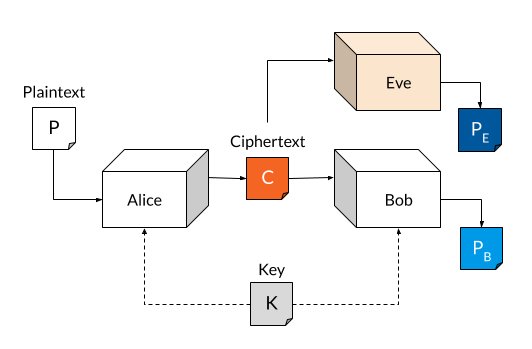
\includegraphics[height=2.5in]{../ref/anc.png}
  \end{center}

  \begin{abstract}
    In this project, we demonstrate that neural networks can learn to protect communications, 
    and build a network which can encrypt and decrypt bit-strings.
    The learning does not require prescribing a particular set of cryptographic algorithms, 
    nor indicating ways of applying these algorithms. We do not prescribe specific
    cryptographic algorithms to these neural networks; instead, we train end-to-end,
    adversarially. We demonstrate that the neural networks can learn how to perform
    forms of encryption and decryption, and also how to apply these operations selectively
    in order to meet confidentiality goals.
  \end{abstract}

  \section{Introduction} 
  As neural networks are applied to increasingly complex tasks, they are often trained to meet end-to-end 
  objectives that go beyond simple functional specifications. These objectives include, for
  example, generating realistic images\cite{gans} and solving multiagent problems. 

  Cryptography is broadly concerned with algorithms and protocols that ensure the secrecy and integrity
  of information. Cryptographic mechanisms are typically described as programs or Turing
  machines. Attackers are also described in those terms, with bounds on their complexity 
  and on their chances of success. A mechanism is deemed secure if it achieves its goal 
  against all attackers. For instance, an encryption algorithm is said to be secure if 
  no attacker can extract information about plaintexts from ciphertexts.
  Modern cryptography provides rigorous versions of such definitions.

  Neural networks are generally not meant to be great at cryptography. Famously, the simplest neural
  networks cannot even compute XOR, which is basic to many cryptographic algorithms. Nevertheless,
  as was demonstrated in the seminal paper on this subject\cite{seminalanc} by Abadi et. al in 2016,
  neural networks can learn to protect the confidentiality of their data from
  other neural networks: they discover forms of encryption and decryption, without being taught 
  specific algorithms for these purposes.

  Knowing how to encrypt is seldom enough for security and privacy. Interestingly, neural networks
  can also learn what to encrypt in order to achieve a desired secrecy property while maximizing
  utility. Thus, when we wish to prevent an adversary from seeing a fragment of a plaintext, or from
  estimating a function of the plaintext, encryption can be selective, hiding the plaintext only partly.

    \subsection{Objective}
    The goal of this {\bfseries Minor Project} is to examine concept of Adversarial Neural 
    Cryptography and implement the algorithms and models described in the relevant literature.
    Advancing these lines of work, we show that neural networks can learn to protect their 
    communications in order to satisfy a policy specified in terms of an adversary.
    The resulting cryptosystems are generated automatically by learning to prevent an adversary
    from learning information about the transmission.

    From the perspective of cryptography, it relates to big themes such as privacy and 
    discrimination. While we embrace a playful, exploratory  approach, we do so with the 
    hope that it will provide insights useful for further work on these topics.
    
    \subsection{Literature Review}
    Classical cryptography may be able to support some applications along these lines. In particular,
    homomorphic encryption enables inference on encrypted data (Xie et al, 2014; Gilad-Bachrach
    et al, 2016).

    Prior work at the intersection of machine learning and cryptography has focused on the 
    generation and establishment of cryptographic keys \cite{netsync}, and on corresponding
    attacks (Klimov et al, 2002). In contrast, our work takes these keys for granted, and 
    focuses on their use; a crucial, new element in our work is the reliance on adversarial 
    goals and training. 

    More broadly, from the perspective of machine learning, our work relates to the application of 
    neural networks to multiagent tasks, mentioned above, and to the vibrant research on 
    generative models and on adversarial training (Denton et al, 2015; 
    Salimans et al, 2016; Nowozin et al, 2016; Chen et al, 2016; Ganin et al, 2015).

      \subsubsection{Inferences from Review}
      \begin{itemize}
        \item It is possible to synchronize two networks while being loosely connected.
        \item It is possible to use GANs such that they are able to encrypt text.  
        \item An agent will only be as strong as the environment it's put in. 
        \item Although a NN might not be able to decipher an encrypted message, 
        it might be trivial for a human. 
      \end{itemize}

  % -------------------------------------------------------
  \newpage 
  \section{Adversarial Neural Networks}
  The concept of {\bfseries adversarial learning} comes from the field of {\bfseries Game Theory,} the branch of 
  mathematics concerned with the analysis of strategies for dealing with competitive situations 
  where the outcome of a participant's choice of action depends critically on the actions 
  of other participants. Game theory has been applied to contexts in war, business, and biology.

    \subsection{The Nash equilibrium}
    Consider a game between two adversaries. In this simple game, both players can choose strategy A, 
    to receive a fixed reward, or strategy B, to receive a fixed penalty. 
    Logically, both players choose strategy A and receive a reward. If you revealed one's strategy 
    to the other and vice versa, you see that no player deviates from the original choice. Knowing the other player's move means little 
    and doesn't change either player's behaviour. This outcome represents a {\bfseries Nash equilibrium.}

    Nash equilibrium is named after its inventor, John Nash, an American mathematician. 
    It is considered one of the most important concepts of game theory, which attempts to 
    determine mathematically and logically the actions that participants of a game should 
    take to secure the best outcomes for themselves. 

    \subsection{Generative Adversarial Networks}
    Generative Adversarial Networks, or GANs for short, are an approach to generative modelling 
    using deep learning methods, such as convolutional neural networks.

    GANs are based on the concept of Nash Equilibrium in that the method of training a network
    isnt derived from labelled data, but from a process of trying to win against another neural
    network. The system consists of a {\bfseries Generator} and a {\bfseries Discriminator} which
    are two neural networks.

    The Generator $G$ produces a fake sample $G(z)$ from a noise sample $z$.
    The Discriminator $D$ is given the fake and real samples $G(z)$ and $x$ randomly and has to
    output a probability which says how likely is it that the current example is fake.

    \begin{figure}[H]
      \centering
      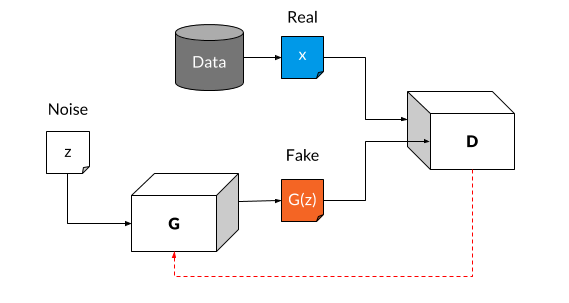
\includegraphics[height=2.5in]{../ref/basicgan.png}
      \caption{Basic GAN}
      \label{fig:basicgan}
    \end{figure}

    The loss of the discriminator (i.e. how wrong $D$ is at finding a fake) is what drives the 
    learning of the generator. If the discriminator is very good at finding a fake, the generator 
    has to work harder and harder to produce a better fake that can fool the discriminator. This
    makes the generator very good at producing fakes. After the training, the discriminator is usually
    discarded and the generator is used by itself.

    The adversarial modelling framework is most straightforward to apply when the models are both
    multilayer perceptrons. To learn the generator’s distribution $p_{g}$ over data $x$, we define a prior on
    input noise variables $p_{z}(z)$, then represent a mapping to data space as $G(z; \theta_{g})$, where $G$ is a
    differentiable function represented by a multilayer perceptron with parameters $\theta_{g}$. We also define a
    second multilayer perceptron $D(x; \theta_{d})$ that outputs a single scalar. $D(x)$ represents the probability
    that $x$ came from the data rather than $p_{g}$. 
    
    We train $D$ to maximize the probability of assigning the
    correct label to both training examples and samples from $G$. We simultaneously train $G$ to minimize
    $log(1 - D(G(z)))$. In other words, $D$ and $G$ play the following two-player 
    {\bfseries minimax game} with value function

    \[ V(G,D)_{minGmaxD} = \mathbb{E}_{x \sim p(x)} \log D(x) + \mathbb{E}_{z \sim Q(z)} \log [1 - D(G(z))] \]

    GANs are a clever way of training a generative model by framing the problem as a 
    supervised learning problem with two sub-models: the generator model that we train to 
    generate new examples, and the discriminator model that tries to classify examples as 
    either real (from the domain) or fake (generated). The two models are trained together in 
    a zero-sum game, adversarial, until the discriminator model is fooled about half the time, 
    meaning the generator model is generating plausible examples.

    GANs are an exciting and rapidly changing field, delivering on the promise of generative 
    models in their ability to generate realistic examples across a range of problem domains, 
    most notably in image-to-image translation tasks such as translating photos of summer to 
    winter or day to night, and in generating photorealistic photos of objects, scenes, and 
    people that even humans cannot tell are fake.
    
  
  % -------------------------------------------------------
  \newpage 
  \section{Basics of Cryptography}
  Modern cryptography is heavily based on mathematical theory and computer science practice; 
  cryptographic algorithms are designed around computational hardness assumptions, making such 
  algorithms hard to break in practice by any adversary. It is theoretically possible to break 
  such a system, but it is infeasible to do so by any known practical means. These schemes are 
  therefore termed computationally secure; theoretical advances, e.g., improvements in integer 
  factorization algorithms, and faster computing technology require these solutions to be 
  continually adapted. There exist information-theoretically secure schemes that provably 
  cannot be broken even with unlimited computing power—an example is the one-time pad—but 
  these schemes are more difficult to use in practice than the best theoretically breakable 
  but computationally secure mechanisms.

  Until modern times, cryptography referred almost exclusively to {\bfseries encryption}, 
  which is the process of converting ordinary information (called plaintext) into unintelligible form 
  (called ciphertext). {\bfseries Decryption} is the reverse, in other words, moving from the 
  unintelligible ciphertext back to plaintext. 
  
  {\bfseries A cipher} is a pair of algorithms that create the encryption and the reversing 
  decryption. The detailed operation of a cipher is controlled both by the algorithm and 
  in each instance by a "key". The key is a secret (ideally known only to the communicants), 
  usually a short string of characters, which is needed to decrypt the ciphertext. 
  
  Formally, a "cryptosystem" is the ordered list of elements of finite possible plaintexts, 
  finite possible cyphertexts, finite possible keys, and the encryption and decryption 
  algorithms which correspond to each key. Keys are important both formally and in actual 
  practice, as ciphers without variable keys can be trivially broken with only the knowledge 
  of the cipher used and are therefore useless (or even counter-productive) for most purposes.

    \subsection{Public Key Encryption}
    Public-key cryptography, or asymmetric cryptography, is a cryptographic system that uses 
    pairs of keys: public keys, which may be disseminated widely, and private keys, which are 
    known only to the owner. The generation of such keys depends on cryptographic algorithms 
    based on mathematical problems to produce one-way functions. Effective security only 
    requires keeping the private key private; the public key can be openly distributed 
    without compromising security.

    \begin{figure}[H]
      \centering
      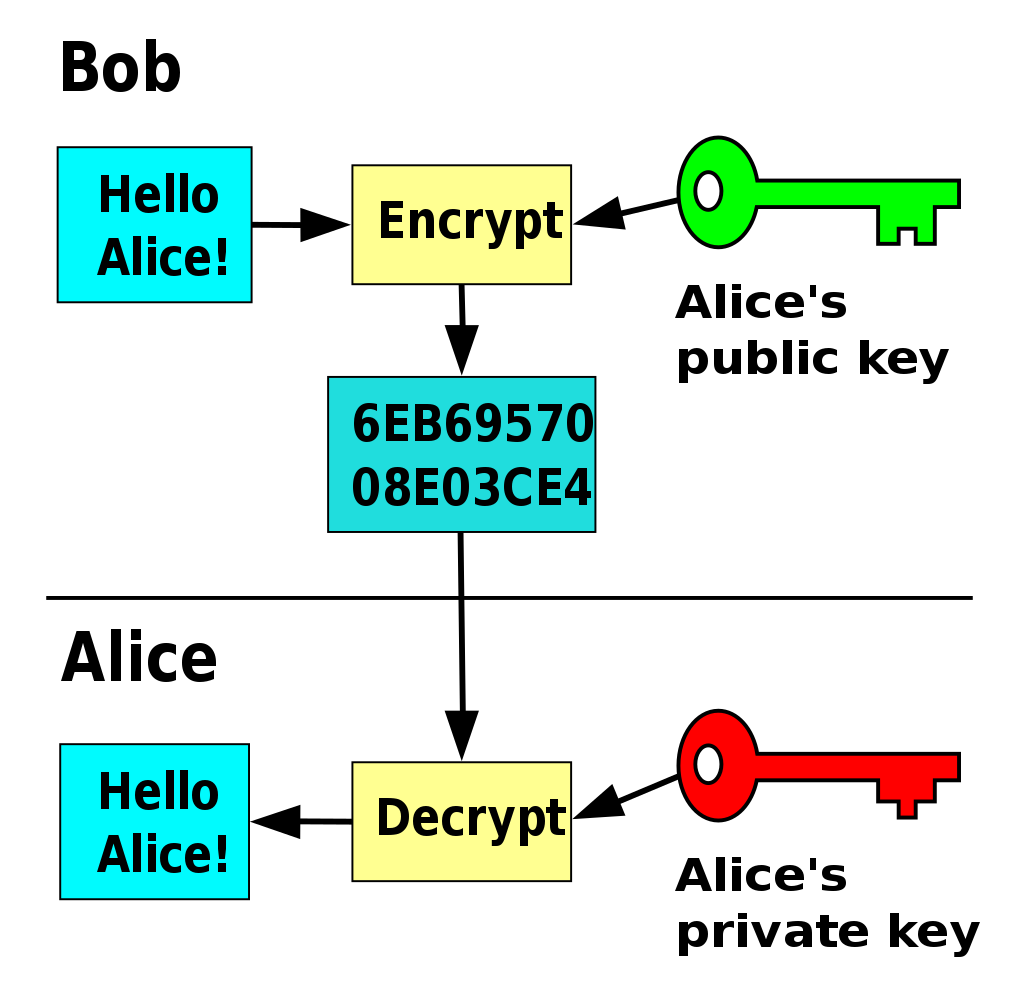
\includegraphics[height=2.5in]{../ref/publickey.png}
      \caption{Public Key Encryption mechanism}
      \label{fig:publickey}
    \end{figure}

    In such a system, any person can encrypt a message using the receiver's public key, 
    but that encrypted message can only be decrypted with the receiver's private key. 
    This allows, for instance, a server to generate a cryptographic key intended for 
    symmetric-key cryptography, then use a client's openly-shared public key to encrypt 
    that newly-generated symmetric key. Now, the server can send this encrypted symmetric 
    key on insecure channels to the client, and only the client can decrypt it using 
    the client's private key pair to the public key used by the server to encrypt this 
    message. With the client and server both having the same symmetric key now, they 
    can safely transition to symmetric key encryption to securely communicate back and 
    forth on otherwise-insecure channels. This has the advantage of not having to manually 
    pre-share symmetric keys, while also gaining the higher data throughput advantage of 
    symmetric-key cryptography over asymmetric key cryptography.

    With public-key cryptography, robust authentication is also possible. 
    A sender can combine a message with a private key to create a short digital signature 
    on the message. Anyone with the sender's corresponding public key can combine the same 
    message and the supposed digital signature associated with it to verify whether the 
    signature was valid, i.e. made by the owner of the corresponding private key.

    \subsection{Symmetric Key Encryption}
    Symmetric-key cryptography refers to encryption methods in which both the sender and 
    receiver share the same key (or, less commonly, in which their keys are different, but 
    related in an easily computable way).

    \begin{figure}[H]
      \centering
      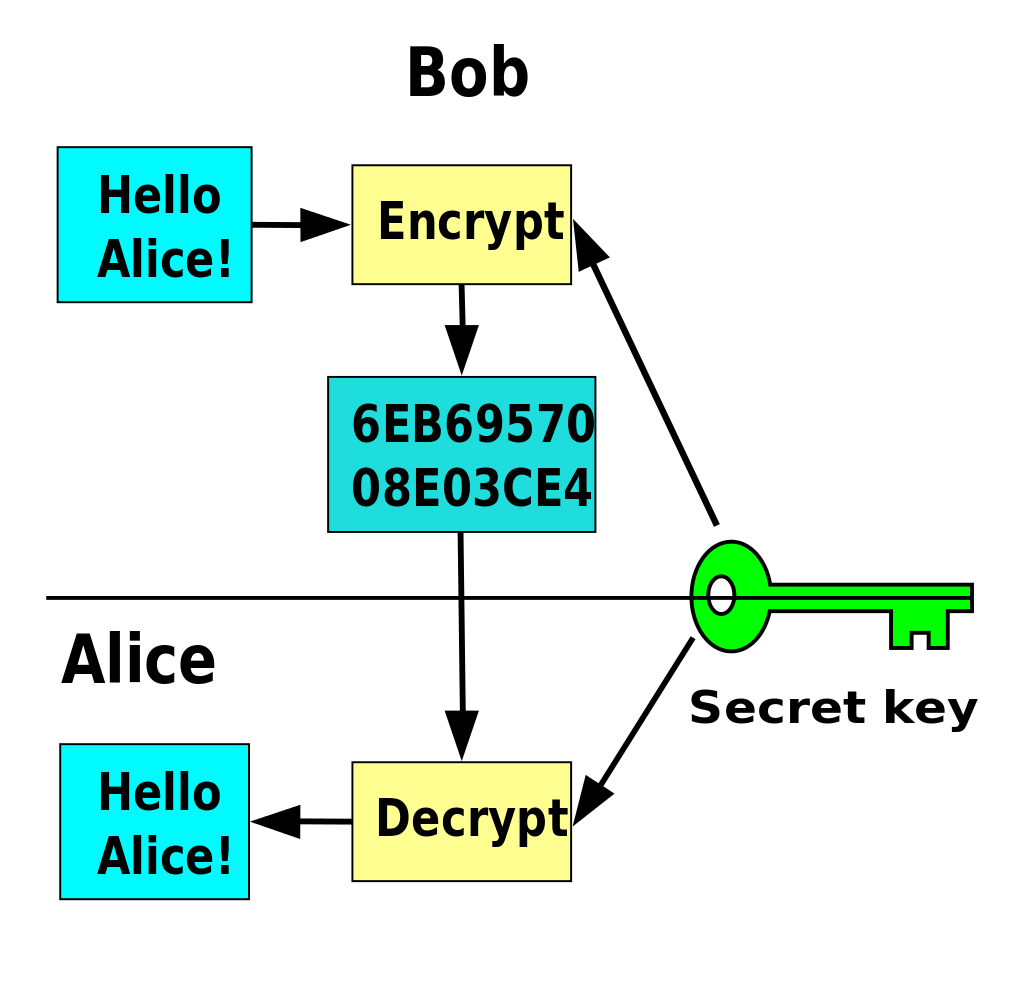
\includegraphics[height=2.5in]{../ref/symmetrickey.png}
      \caption{Symmetric Key Encryption mechanism}
      \label{fig:symmetrickey}
    \end{figure}
    
    Symmetric key ciphers are implemented as either block ciphers or stream ciphers. 
    A block cipher enciphers input in blocks of plaintext as opposed to individual characters, 
    the input form used by a stream cipher.

    {\bfseries Cryptographic hash functions} are a third type of cryptographic algorithm. 
    They take a message of any length as input, and output a short, fixed length hash, which 
    can be used in (for example) a digital signature. For good hash functions, an attacker 
    cannot find two messages that produce the same hash. MD4 is a long-used hash function 
    that is now broken; MD5, a strengthened variant of MD4, is also widely used but broken 
    in practice. Cryptographic hash functions are used 
    to verify the authenticity of data retrieved from an untrusted source or to add a layer 
    of security.
    
    The US National Security Agency developed the Secure Hash Algorithm series of MD5-like 
    hash functions: SHA-0 was a flawed algorithm that the agency withdrew; SHA-1 is widely 
    deployed and more secure than MD5, but cryptanalysts have identified attacks against it; 
    the SHA-2 family improves on SHA-1, but is vulnerable to clashes as of 2011; and the US 
    standards authority thought it "prudent" from a security perspective to develop a new 
    standard to "significantly improve the robustness of NIST's overall hash algorithm toolkit."
    \cite{neuralhash}
    Thus, a hash function design competition was meant to select a new U.S. national standard, 
    to be called SHA-3, by 2012. 
    
    The competition ended on October 2, 2012 when the NIST 
    announced that Keccak would be the new SHA-3 hash algorithm. Unlike block and stream 
    ciphers that are invertible, cryptographic hash functions produce a hashed output that 
    cannot be used to retrieve the original input data. 

    \subsection{One Time Pad Algorithm}
    In cryptography, the one-time pad (OTP) is an encryption technique that cannot be cracked, 
    but requires the use of a one-time pre-shared key the same size as, or longer than, the message 
    being sent. In this technique, a plaintext is paired with a random secret key (also referred 
    to as a one-time pad). Then, each bit or character of the plaintext is encrypted by combining 
    it with the corresponding bit or character from the pad using modular addition.

    The resulting ciphertext will be impossible to decrypt\cite{otpinvent} or break if the following 
    four conditions are met:
    \begin{itemize}
      \item The key must be truly random.
      \item The key must be at least as long as the plaintext.
      \item The key must never be reused in whole or in part.
      \item The key must be kept completely secret.
    \end{itemize}

    It has also been proven that any cipher with the property of perfect secrecy must use keys 
    with effectively the same requirements as OTP keys. Digital versions of one-time pad 
    ciphers have been used by nations for critical diplomatic and military communication, 
    but the problems of secure key distribution have made them impractical for most applications.

    \subsection{Neural Cryptography}
    {\bfseries Neural cryptography} is a branch of cryptography dedicated to analyzing the 
    application of stochastic algorithms, especially artificial neural network algorithms, 
    for use in encryption and cryptanalysis.

    Artificial neural networks are well known for their ability to selectively explore the 
    solution space of a given problem. This feature finds a natural niche of application in 
    the field of cryptanalysis. At the same time, neural networks offer a new approach to attack 
    ciphering algorithms based on the principle that any function could be reproduced by a 
    neural network, which is a powerful proven computational tool that can be used to find 
    the inverse-function of any cryptographic algorithm.

    The ideas of mutual learning, self learning, and stochastic behavior of neural networks 
    and similar algorithms can be used for different aspects of cryptography, like public-key 
    cryptography, solving the key distribution problem using neural network mutual 
    synchronization, hashing or generation of pseudo-random numbers.

    Another idea is the ability of a neural network to separate space in non-linear pieces 
    using "bias". It gives different probabilities of activating the neural network or not. 
    This is very useful in the case of Cryptanalysis. 
    Two names are used to design the same domain of research: Neuro-Cryptography and Neural 
    Cryptography.

      \subsubsection{Neural key exchange protocol}
      The most used protocol for key exchange between two parties A and B in the practice 
      is Diffie–Hellman key exchange protocol. Neural key exchange, which is based on the 
      synchronization of two tree parity machines, should be a secure replacement for this method. 
      Synchronizing these two machines is similar to synchronizing two chaotic oscillators 
      in chaos communications.

      \pagebreak
      Each party (A and B) uses its own {\bfseries tree parity machine.} 
      The tree parity machine is a special type of multi-layer feedforward neural network.
      Synchronization of the tree parity machines is achieved in these steps
      \begin{enumerate}
        \item Initialize random weight values
        \item Execute these steps until the full synchronization is achieved
        \begin{enumerate}
          \item Generate random input vector X
          \item Compute the values of the hidden neurons
          \item Compute the value of the output neuron
          \item Compare the values of both tree parity machines
          \begin{enumerate}
            \item Outputs are the same: go to 2(a)
            \item Outputs are different: one of the suitable learning rules is applied to the weights
          \end{enumerate}
        \end{enumerate}
      \end{enumerate}

      The following {\bfseries Hebbian learning rule} can be used for the synchronization

      \[ w_{i}^+ = g( w_{i} + {\sigma}_{i}x_{i} {\Theta}({\sigma}_{i}{\tau}) {\Theta}({\tau}^A{\tau}^B) ) \]

      After the full synchronization is achieved (the weights $w_{ij}$ of both tree 
      parity machines are same), A and B can use their weights as keys.
      This method is known as a bidirectional learning.\cite{netsync}

      The synchronized weights
      are used to construct an ephemeral key exchange protocol for a secure
      transmission of secret data. It is shown that an opponent who knows
      the protocol and all details of any transmission of the data has no
      chance to decrypt the secret message, since tracking the weights is a
      hard problem compared to synchronization\cite{netsync}. The complexity of the
      generation of the secure channel is linear with the size of the network. 

  % -------------------------------------------------------
  \newpage 
  \section{Adversarial Neural Cryptography}
  This section discusses how to protect the confidentiality of plaintexts using shared keys. It describes
  the organization of the system that we consider, and the objectives of the participants in this system.
  It also explains the training of these participants, defines their architecture, and presents experiments.

  A classic scenario in security involves three parties: Alice, Bob, and Eve. Typically, Alice and Bob
  wish to communicate securely, and Eve wishes to eavesdrop on their communications. Thus, the
  desired security property is secrecy (not integrity), and the adversary is a “passive attacker” that
  can intercept communications but that is otherwise quite limited: it cannot initiate sessions, inject
  messages, or modify messages in transit.

    \subsection{The ANC Model}
    We start with a particularly simple instance of this scenario, 
    depicted in figure \ref{fig:anc}, in which Alice
    wishes to send a single confidential message P to Bob. The message P is an input to Alice. When
    Alice processes this input, it produces an output C. (“P” stands for “plaintext” and “C” stands for
    “ciphertext”). Both Bob and Eve receive C, process it, and attempt to recover P. We represent what
    they compute by $P_{Bob}$ and $P_{Eve}$, respectively. 
    
    Alice and Bob have an advantage over Eve: they share
    a secret key K\cite{seminalanc}. We treat K as an additional input to Alice and Bob. We assume one fresh key K per
    plaintext P, but, at least at this abstract level, we do not impose that K and P have the same length.
    
    \begin{figure}[H]
      \centering
      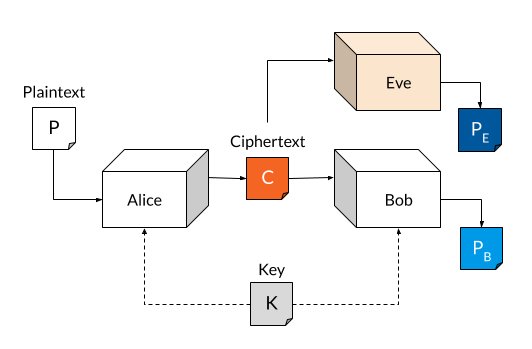
\includegraphics[height=2.5in]{../ref/anc.png}
      \caption{The ANC Model proposed by Abadi et al.}
      \label{fig:anc}
    \end{figure}    
    
    For us, Alice, Bob, and Eve are all neural networks. We describe their structures in Section \ref{sec:anc_netarch}. 
    They each have parameters, which we write $\Phi_{A}$, $\Phi_{B}$, and $\Phi_{E}$, respectively. Since $\Phi_{A}$ and
    $\Phi_{B}$ need not be equal, encryption and decryption need not be the same function even if Alice and
    Bob have the same structure. As is common for neural networks, Alice, Bob, and Eve work over
    tuples of floating-point numbers, rather than sequences of bits. In other words, K, P, PBob, PEve,
    and C are all tuples of floating-point numbers. Note that, with this formulation, C, $P_{Bob}$, and $P_{Eve}$
    may consist of arbitrary floating-point numbers even if P and K consist of 0s and 1s. 
    
    This set-up, although rudimentary, suffices for basic schemes, in particular allowing for the possibility
    that Alice and Bob decide to rely on K as a one-time pad, performing encryption and decryption
    simply by XORing the key K with the plaintext P and the ciphertext C, respectively. However,
    we do not require that Alice and Bob function in this way—and indeed, in our experiments in
    Section 2.5, they discover other schemes. For simplicity, we ignore the process of generating a key
    from a seed. We also omit the use of randomness for probabilistic encryption. 
    Such enhancements may be the subject of further work.

      \subsubsection{Objectives of the Participants}
      Informally, the objectives of the participants are as follows. Eve’s goal is simple: to reconstruct P
      accurately (in other words, to minimize the error between P and $P_{Eve}$). Alice and Bob want to communicate
      clearly (to minimize the error between P and PBob), but also to hide their communication
      from Eve. Note that, in line with modern cryptographic definitions (Goldwasser \& Micali,
      1984), we do not require that the ciphertext C “look random” to Eve. A ciphertext may even contain
      obvious metadata that identifies it as such. Therefore, it is not a goal for Eve to distinguish C
      from a random value drawn from some distribution. In this respect, Eve’s objectives contrast with
      common ones for the adversaries of GANs. On the other hand, one could try to reformulate Eve’s
      goal in terms of distinguishing the ciphertexts constructed from two different plaintexts.

    Much as in the definitions of GANs, we would like Alice and Bob to defeat the best
    possible version of Eve, rather than a fixed Eve. Of course, Alice and Bob may not win for every
    plaintext and every key, since knowledge of some particular plaintexts and keys may be hardwired
    into Eve. (For instance, Eve could always output the same plaintext, and be right at least once.)
    Therefore, we assume a distribution on plaintexts and keys, and phrase our goals for Alice and Bob
    in terms of expected values.

      \subsubsection{Mathematical Background}
      We write $A(\Phi_{A}, P,K)$ for Alice’s output on input $P,K$, write $B(\Phi_{B},C,K)$ for Bob’s output on
      input $C,K$, and write $E(\Phi_{E},C)$ for Eve’s output on input $C$. We introduce a distance function d on
      plaintexts. 
      
      Although the exact choice of this function is probably not crucial, for concreteness we
      take the L1 distance 
        
      \[ d(P, P^\prime) = \Sigma_{i=1}^N | P_{i} - P_{i}^\prime | \]
      
      where N is the length of plaintexts. 
      We define a per-example loss function for Eve.
      Intuitively this represents how much Eve is wrong when the plaintext is P and the
      key is K. We also define a loss function for Eve over the distribution on plaintexts and keys by
      taking an expected value:

      \[ L_{E}(\Phi_{A}, \Phi_{E}) = \mathbb{E}_{P,K} [ d(P, E(\Phi_{E}, A(\Phi_{A},  P, K))) ] \]

      We obtain the “optimal Eve” by minimizing this loss:
      
      \[ O_{E}(\theta_{A}) = argmin_{\theta_{E}}(L_{E}(\theta_{A}, \theta_{E})) \]

      Similarly, we define a per-example reconstruction error for Bob, and extend it to the 
      distribution on plaintexts and keys. We define a loss function for Alice and Bob by 
      combining $L_{B}$ and the optimal value of $L_{E}$:
      
      \[ L_{AB}(\Phi_{A}, \Phi_{E}) = L_{B}(\Phi_{A}, \Phi_{B}) - L_{E}(\Phi_{A}, O_{E}(\theta_{A})) \]
      
      This combination reflects that Alice and Bob want to minimize Bob’s reconstruction error and to
      maximize the reconstruction error of the “optimal Eve”. The use of a simple subtraction is somewhat
      arbitrary; below we describe useful variants. We obtain the “optimal Alice and Bob” by minimizing
      
      \[ (O_{A}, O_{B}) = argmin_{(\theta_{A}, \theta_{B})}(L_{AB}(\theta_{A}, \theta_{B})) \]
      
      We write “optimal” in quotes because there need be no single global minimum. In general, there
      are many equi-optimal solutions for Alice and Bob. As a simple example, assuming that the key is
      of the same size as the plaintext and the ciphertext, Alice and Bob may XOR the plaintext and the
      ciphertext, respectively, with any permutation of the key, and all permutations are equally good as
      long as Alice and Bob use the same one; moreover, with the way we architect our networks (see
      Section 2.4), all permutations are equally likely to arise.

      \subsubsection{Network Architecture} \label{sec:anc_netarch}
      The Architecture of Alice, Bob, and Eve Because we wish to explore whether a general neural
      network can learn to communicate securely, rather than to engineer a particular method, we aimed
      to create a neural network architecture that was sufficient to learn mixing functions such as XOR,
      but that did not strongly encode the form of any particular algorithm.
      To this end, we chose the following “mix \& transform” architecture. It has a first fully-connected
      (FC) layer, where the number of outputs is equal to the number of inputs. The plaintext and key
      bits are fed into this FC layer. Because each output bit can be a linear combination of all of the
      input bits, this layer enables—but does not mandate—mixing between the key and the plaintext bits.
      In particular, this layer can permute the bits. 

      \begin{figure}[H]
        \centering
        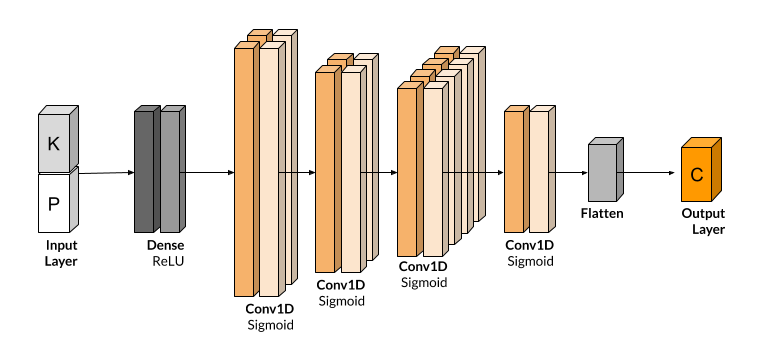
\includegraphics[width=\textwidth]{../ref/anclayers.png}
        \caption{Modified network Model from Abadi et al.}
        \label{fig:anclayers}
      \end{figure}
      
      The FC layer is followed by a sequence of convolutional
      layers, the last of which produces an output of a size suitable for a plaintext or ciphertext.
      These convolutional layers learn to apply some function to groups of the bits mixed by the previous
      layer, without an a priori specification of what that function should be. Notably, the opposite order
      (convolutional followed by FC) is much more common in image-processing applications. Neural
      networks developed for those applications frequently use convolutions to take advantage of spatial
      locality. 
       
      For neural cryptography, we specifically wanted locality—i.e., which bits to combine—to
      be a learned property, instead of a pre-specified one. While it would certainly work to manually pair
      each input plaintext bit with a corresponding key bit, we felt that doing so would be uninteresting.
      We refrain from imposing further constraints that would simplify the problem. For example, we do
      not tie the parameters $\Phi_{A}$ and $\Phi_{B}$, as we would if we had in mind that Alice and Bob should both
      learn the same function, such as XOR.

    \pagebreak
    \subsection{The Cryptonet Model}
    In this section, we describe a proposed improvement to the ANC methodology using the Chosen-Plaintext
    Attack (CPA) called the CPA-ANC. Additionally, we present a simple NN capable of learning the
    One-Time Pad which will be used to test this new methodology against the traditional ANC.

      \subsubsection{Chosen-Plaintext Attack}
      As we will see in the experiments of Section \ref{sec:implementation}, the problem with the approach 
      proposed in the original ANC work \cite{perfanc} is that {\bfseries Eve's job is too hard.} 
      
      It must decrypt a random message having
      access only to the ciphertext. The consequence is that, under this methodology, Alice and Bob learn to
      communicate with cryptosystems that are not truly secure. Therefore, one can conclude that Alice and
      Bob do not have to do much effort to protect themselves against Eve, leading in insecure cryptosystems.
      It is possible to improve ANC considering a more robust model of security for Alice, Bob and Eve.
      Namely, we will let Eve to mount a CPA. Therefore, to be protected against Eve, Alice and Bob will
      have to find a system secure against the CPA.

      \begin{figure}[H]
        \centering
        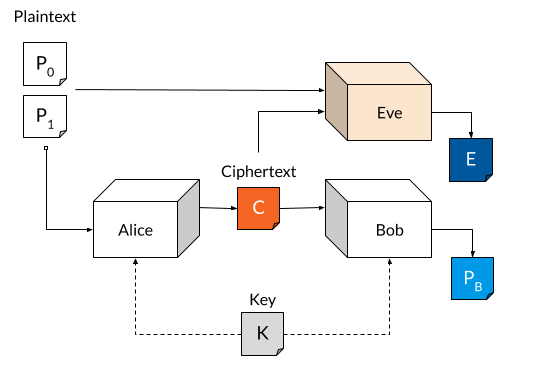
\includegraphics[height=2.5in]{../ref/crnet.png}
        \caption{The Cryptonet Model proposed by Coutinho et al.}
        \label{fig:crnet}
      \end{figure}
      
      In this new setup Eve will choose two messages $P_{0}$ and $P_{1}$ and send them to Alice. Alice will
      choose one of these messages randomly, encrypt it with the NN obtaining the ciphertext C and send
      it to Eve and Bob. As usual, Bob will decrypt the message with a NN. However, Eve will not try to
      decrypt C, but will only output 0 if it believes $P_{0}$ was encrypted or 1 if it believes $P_{1}$ was encrypted.
      We call this the CPA-ANC setup and it is illustrated in Figure \ref{fig:crnet}.

      \subsubsection{Network Architecture} \label{sec:crnet_netarch}

      We are building a NN complex enough to be able to learn some form of cryptography
      but simple enough to allow us to reason about its security. To do this, we used a continuous
      generalization for the operator XOR, which is a well-known binary and non-differentiable operation
      that happens to be used a lot in cryptography. \cite{perfanc}

      Thus, if we want a NN that can perform the XOR operation internally, we need a generalization
      of the operation. It is possible to generalize the XOR operation using the unit circle by mapping the bit
      0 to the angle 0 and the bit 1 to the angle $\pi$. 
      In this way, the XOR is equivalent to the sum of the angles.

      \pagebreak
      Thus, it is possible to work with angles
      different from 0 or p, generalizing bits to a continuous space. The following equation defines the
      mapping of a bit b into an angle:
      
      \[ f(b) = \arccos (1 - 2b) \]
      
      The inverse of f provides the mapping of an angle a to a “continuous bit”:
      
      \[ f^{-1}(a) = \frac{1 - \cos (a)}{2}  \]

      \begin{figure}[H]
        \centering
        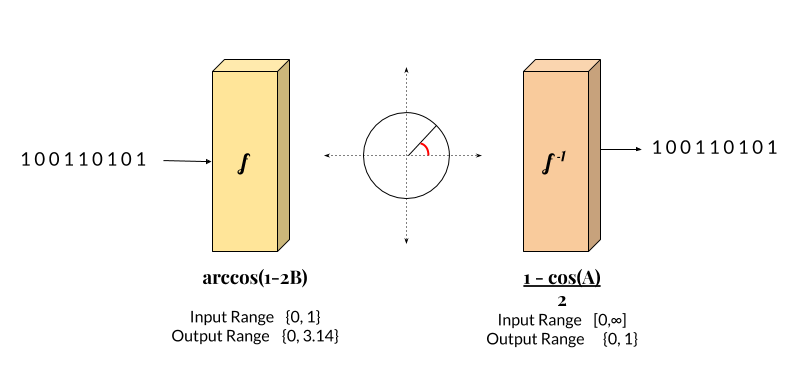
\includegraphics[height=2.5in]{../ref/crnetfunc.png}
        \caption{Transformation Function in Cryptonet}
        \label{fig:crnetfunc}
      \end{figure}

      Basically, CryptoNet receives as input the plaintext and the key and, for each bit received, applies
      the transformation $f(b)$, resulting in angles. The next step is a standard matrix
      multiplication followed by the inverse transformation $f^{-1}(a)$ resulting in the
      ciphertext. Note that the ciphertext is not composed of bits but by floating number between 0 and 1.

      \begin{figure}[H]
        \centering
        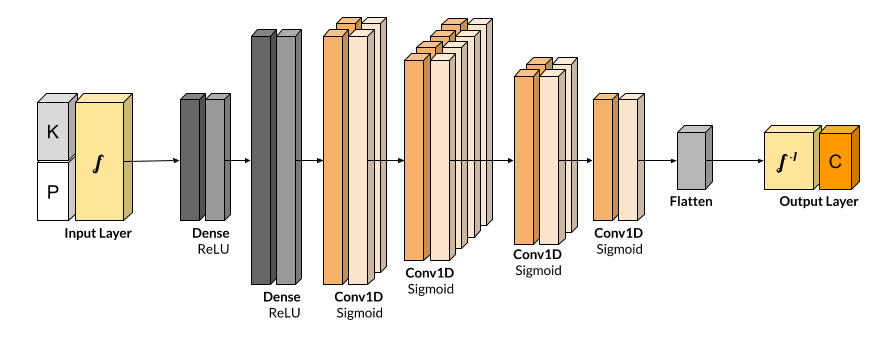
\includegraphics[width=\textwidth]{../ref/crnetlayers.png}
        \caption{Modified network Model from Coutinho et al.}
        \label{fig:crnetlayers}
      \end{figure}

      The realized network model is a hybrid of the two systems considered above. It contains the
      convolutional layers from the original ANC model and applies the transform function and CPA 
      over the top. This is done for reasons of convergence and complexity.
      The original model proposed by Coutinho et al, is a very simple multilayer perceptron and does
      not hold up to large amounts of data. This modified setup helps us incorporate the good things from
      both the versions to produce a better result.
    
  % -------------------------------------------------------
  \newpage 
  \section{Implementation} \label{sec:implementation}
  The implementation of this project was done entirely in {\bfseries Python 3.6} using some popular 
  deep learning libraries and tools to make the work easier. Python was chosen over other languages
  like MATLAB and R since the code is very versatile and relies on open-source software.
  Python is also the language of choice for deployment of ML models in production and is thus ideal.

  The libraries used in this project for the implementation of the network models are
  \begin{itemize}
    \item {\bfseries PyTorch 1.6}; a popular library for functional ML models
    \item {\bfseries Tensorboard}; for visualizations and tracking the training progress
    \item {\bfseries MatPlotLib}; for plotting charts and figures
  \end{itemize}

  Other than these other libraries are used as and when necessary in the code. Further, we will 
  attempt to use the work of Hao Li et al\cite{visualloss} to plot the loss landscape of the 
  high dimensional space of the networks. Other research based 
  software like DeepVis\cite{deepvis} is also used.

    \subsection{Methodology}
    The models that are written were first tested to produce what we call a \\
    {\bfseries successful communication}.
    This means that we run the network without the involvement of an eavesdropper (Eve) and try to
    get Alice and Bob to communicate successfully. This has the effect of synchronizing the two networks.

    We produce a random string of bits as plaintext and use a predetermined key of the same length. 
    These are then concatenated to form the input to the encrypting networks.

    \begin{lstlisting}
      # We use the generator syntax for lists
      KEY = [random.randint(0, 1) for i in range(BLOCKSIZE)]
      PLAIN = [[random.randint(0, 1) for x in range(BLOCKSIZE)] 
        for i in range(BATCHLEN)]

      # ...
      for P in PLAIN:
        P = torch.Tensor(P)
        K = torch.Tensor(KEY)

        torch.cat([P, K], dim=0)
    \end{lstlisting}

    After we have trained the networks for a few epochs without the adversary, we look at the graph
    of the loss plotted over the training batches and a {\bfseries reduction in loss will mean} that
    the communication is successful.

    We then introduce the eavesdropper to the mix and let the networks retrain with it. This has the effect
    of changing the communication scheme learnt by the networks into something more secure. Alice is
    directly affected by the loss of Eve and the better Eve is at predicting the original plaintext, the
    harder Alice has to work to develop a secure cryptosystem.

    \begin{lstlisting}
      # We choose the L1 loss initially
      lossfn = nn.L1Loss()

      bob_reconst_loss = lossfn(Pb, P)
      eve_reconst_loss = lossfn(Pe, P)

      # Linear loss
      alice_loss = bob_reconst_loss - eve_reconst_loss
    \end{lstlisting}

    This system is trained for the remaining epochs and is then tested for its convergence by studying
    it's loss trend over time.

    \subsection{Structure of the Network}
    We have two main structures of network that we have implemented and experimented with. These are
    the original ANC model proposed by Abadi et al \cite{seminalanc} and the second is a hybrid model
    of the improvement proposed by Coutinho et al \cite{perfanc}. This was motivated by poor results
    with the original model proposed and the ambiguity about the network architecture used by the team.

      \subsubsection{ANC Model}
      The model architecture is as described in section \ref{sec:anc_netarch}.

      \begin{figure}[H]
        \centering
        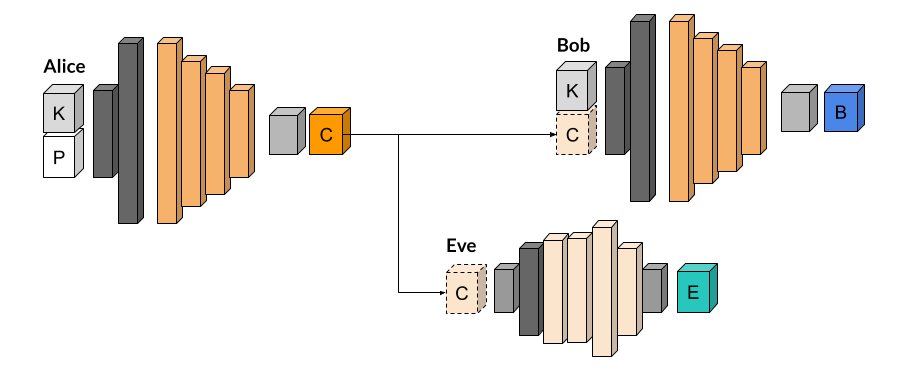
\includegraphics[width=\textwidth]{../ref/ancstruct.png}
        \caption{Network Structure for ANC}
        \label{fig:ancstruct}
      \end{figure}

      \begin{lstlisting}
        class KeyholderNetwork(nn.Module):
          def __init__(self, blocksize):
            super(KeyholderNetwork, self).__init__()
            
            self.blocksize = blocksize
            self.entry = nn.Identity(blocksize * 2)

            self.fc1 = nn.Linear(in_features=blocksize * 2, out_features=blocksize * 2)
            
            self.conv1 = nn.Conv1d(in_c=1, out_c=2, kernel_size=4, stride=1)
            self.conv2 = nn.Conv1d(in_c=2, out_c=2, kernel_size=2, stride=2)
            self.conv3 = nn.Conv1d(in_c=2, out_c=4, kernel_size=1, stride=1)
            self.conv4 = nn.Conv1d(in_c=4, out_c=1, kernel_size=1, stride=1)

          def forward(self, inputs):    
            inputs = self.entry(inputs)
            inputs = torch.sigmoid(self.fc1(inputs))

            inputs = inputs.unsqueeze(0).unsqueeze(0)

            inputs = torch.sigmoid(self.conv1(inputs))
            inputs = torch.sigmoid(self.conv2(inputs))
            inputs = torch.sigmoid(self.conv3(inputs))
            
            inputs = F.hardsigmoid(self.conv4(inputs))

            return inputs.view(self.blocksize)
      \end{lstlisting}

      The last layer of the model was converted to a {\bfseries hardsigmoid} layer. This works
      almost like the sigmoid function but better approximates a discrete output.

      The plaintext and key are converted to PyTorch Tensors which are then concatenated and sent
      to the encrypting networks. For ease of use, the networks that use the key are instances of a 
      {\bfseries KeyholderNetwork} class which takes two {\bfseries BLOCKSIZE} length inputs.
      This allows Alice and Bob to have the same architecture.

      \begin{lstlisting}
        alice = KeyholderNetwork(BLOCKSIZE)
        bob = KeyholderNetwork(BLOCKSIZE)
        eve = AttackerNetwork(BLOCKSIZE)

        lossfn = nn.L1Loss()

        opt_alice_bob = optim.Adam(alice.parameters() + bob.parameters(), lr=0.0008)
        opt_eve = optim.Adam(eve.parameters(), lr=0.0008)

        for E in range(BATCHES):
          for P in PLAIN:
            P = torch.Tensor(P)
            K = torch.Tensor(KEY)

            cipher = alice(torch.cat([P, K], dim=0))
            cipher.detach()

            Pb = bob(torch.cat([cipher, K], dim=0))
            Pe = eve(cipher)

            bob_reconst_loss = lossfn(Pb, P)
            eve_reconst_loss = lossfn(Pe, P)

            # Linear loss
            alice_loss = (BETA * bob_reconst_loss) - (GAMMA * eve_reconst_loss)

            bob_reconst_loss.backward(retain_graph=True)
            eve_reconst_loss.backward(retain_graph=True)
            alice_loss.backward(retain_graph=True)

            opt_alice_bob.step()
            opt_eve.step()

            delta_alice = alice_running_loss[-1] - alice_loss.item()
            delta_bob = bob_running_loss[-1] - bob_reconst_loss.item()
            delta_eve = eve_running_loss[-1] - eve_reconst_loss.item()

            # Stop when no/low avg change
            if ((delta_alice + delta_bob + delta_eve)/3 <= 0.00005):
              print('--- Training Stalled ---')
              break

          print(f'Finished Batch {E}')
          recalc_plain()

        print('Finished Training')
      \end{lstlisting}

      \subsubsection{Cryptonet Model}
      This network has almost the same architecture as the ANC model, but has a few changes.
      The inputs go through a functional transform layer which converts the bits into angles \cite{perfanc}.
      
      The layer sizes have been changed by experimental inference and have been found to work better in
      the configuration illustrated in the figure \ref{fig:crnetlayers}.

      \begin{figure}[H]
        \centering
        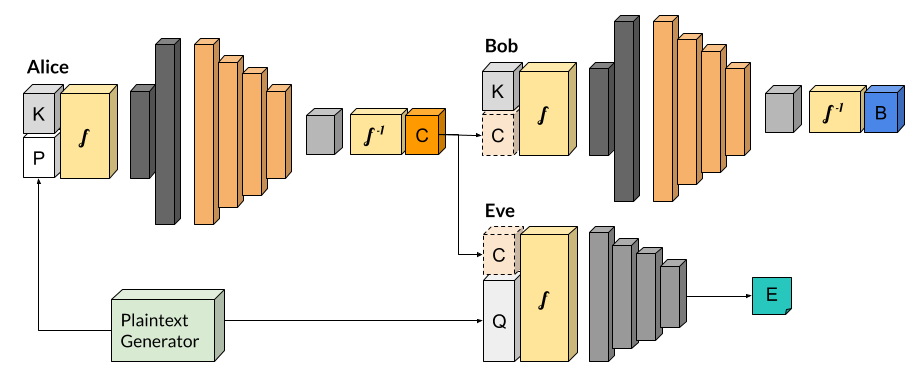
\includegraphics[width=\textwidth]{../ref/crnetstruct.png}
        \caption{Network Structure for Cryptonet}
        \label{fig:crnetstruct}
      \end{figure}

      \begin{lstlisting}
        class KeyholderNetwork(nn.Module):
          def __init__(self, blocksize):
            super(KeyholderNetwork, self).__init__()
            self.entry = nn.Identity(blocksize * 2)

            self.fc1 = nn.Linear(in_features=blocksize * 2, out_features=blocksize * 4)
            self.fc2 = nn.Linear(in_features=blocksize * 4, out_features=blocksize * 2)
            self.fc3 = nn.Linear(in_features=blocksize, out_features=blocksize)
            
            # ... Same conv layers as in ANC

          def forward(self, inputs):    
            inputs = self.entry(inputs)
            inputs = torch.acos(1 - torch.mul(inputs, 2))

            inputs = torch.relu(self.fc1(inputs))
            inputs = torch.relu(self.fc2(inputs))

            inputs = inputs.unsqueeze(dim=0).unsqueeze(dim=0)
            
            inputs = torch.sigmoid(self.conv1(inputs))
            inputs = torch.sigmoid(self.conv2(inputs))
            inputs = torch.sigmoid(self.conv3(inputs))
            inputs = torch.sigmoid(self.conv4(inputs))
            
            inputs = inputs.view(self.blocksize)
            inputs = torch.relu(self.fc3(inputs))

            inputs = torch.div(1 - torch.cos(inputs), 2)
            inputs = F.hardsigmoid(torch.mul(inputs, 10) - 5)

            return inputs
      \end{lstlisting}

      Similar to the ANC model, the inputs are concatenated before being sent to Alice.
      However, the plaintext is randomly chosen from one of two pre-generated plaintexts.
      Eve is given both the plaintexts and the ciphertext and has to determine if the cipher
      was produced either from $P_{0}$ or $P_{1}$. Its output is a probability between 0 and 1.

      Here we also train the model for half of the epoch without the involvement of Eve, i.e. not 
      training Eve and not backpropagating its loss, while for the other half we have Eve in the system.

      It was also noted from experimentation that the {\bfseries Mean Squared Error Loss (L2 Loss)} works better in this
      scenario. We also experimented with {\bfseries Binary Crossentropy Loss} but without significantly better results.

      \begin{lstlisting}
        # Initialize Networks
        alice = KeyholderNetwork(BLOCKSIZE)
        bob = KeyholderNetwork(BLOCKSIZE)
        eve = AttackerNetwork(BLOCKSIZE)

        dist = nn.MSELoss()
        # dist = nn.BCELoss()

        ab_params = itertools.chain(alice.parameters(), bob.parameters())
        opt_alice_bob = torch.optim.Adam(ab_params, lr=1e-3, weight_decay=1e-5)

        opt_eve = torch.optim.Adam(eve.parameters(), lr=2e-4)
        
        # Training loop
        torch.autograd.set_detect_anomaly(True)

        for E in range(EPOCHS):
          print(f'Epoch {E + 1}/{EPOCHS}')
          K = torch.Tensor(KEY)

          for B in range(BATCHES):
            for X in PLAIN:
              P0 = torch.Tensor(X[0])
              P1 = torch.Tensor(X[1])

              R = random.randint(0, 1)
              P = torch.Tensor(X[R])
                    
              C = alice(torch.cat([P, K], dim=0))
              Pb = bob(torch.cat([C, K], dim=0))

              # Loss and BackProp
              bob_dec_loss = dist(Pb, P)
              opt_alice_bob.zero_grad()

              if B > BATCHES/2:
                Re = eve(torch.cat([P0, P1, C.detach()], dim=0))
                eve_adv_loss = dist(Re, torch.Tensor([1 - R, R]))
                bob_dec_loss = dist(Pb, P) + torch.square(1 - eve_adv_loss)
              
                bob_dec_loss.backward(retain_graph=True)
                opt_alice_bob.step()

                opt_eve.zero_grad()
                eve_adv_loss.backward(retain_graph=True)
                opt_eve.step()
              else:
                bob_dec_loss.backward(retain_graph=True)
                opt_alice_bob.step()
      \end{lstlisting}

    \subsection{Training}
    The training for this network is accomplished, as stated before, by first training without
    the eavesdropper so that the communication can be established. This ensures that the Alice and
    Bob neural networks are synchronized before introducing Eve. After a few epochs, we introduce
    Eve to the system and let the training complete, which watching the training loss.

    We have used the {\bfseries Adam Optimizer} which handles the backpropagation steps in the
    training of the networks. The Adam optimization algorithm is an extension to stochastic 
    gradient descent that has recently seen broader adoption for deep learning applications 
    in computer vision and natural language processing. Instead of adapting the parameter 
    learning rates based on the average first moment (the mean) as in RMSProp, Adam also 
    makes use of the average of the second moments of the gradients (the uncentered variance).

    \begin{figure}[H]
      \centering
      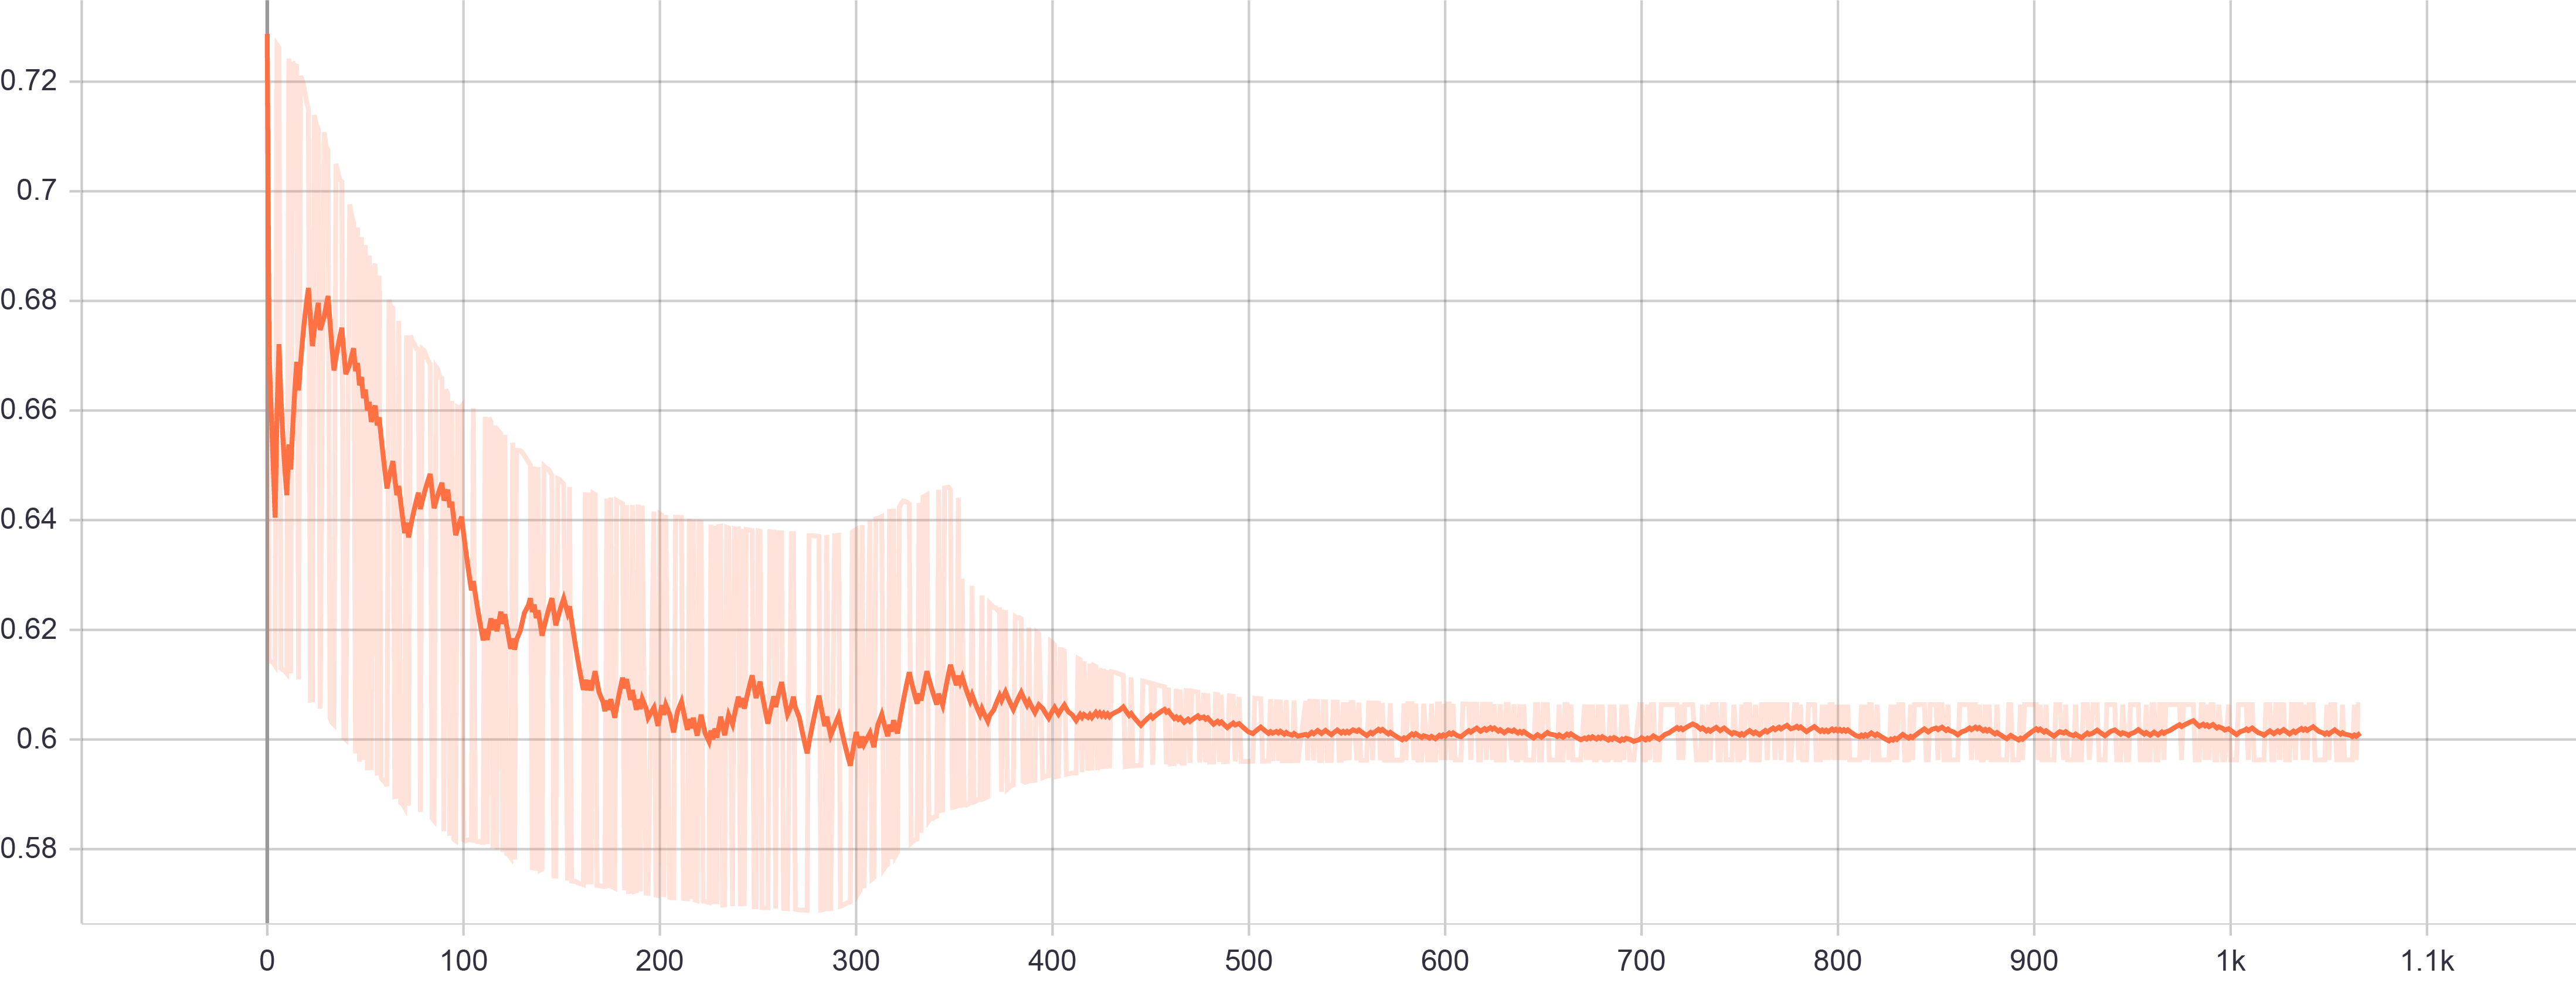
\includegraphics[height=2in]{../../models/cryptonet/graphs/TrainingLoss[S].png}
      \caption{Training Loss Trend with Cryptonet}
      \label{fig:trn_crnet}
    \end{figure} 

    The loss while training is recorded using Tensorboard and this helps us keep an eye on the
    gradients and allows us to detect a stalled training and stop.

      \subsubsection{Training Parameters}
      The parameters which aren't learnt by the network but directly affect the performance are
      called {\bfseries hyperparameters}. These are important since the right choice of hyperparameters
      can get us to the optimal model very quickly.

      For our purposes the important parameters are the {\bfseries key length, learning rate and the
      loss coefficients} in calculation of the loss for Alice and Bob. Various combinations are tried
      until one good set of values is obtained by experimentation.      

      The following table lists the various values of the hyperparameters that were tried and
      produced some useful results.

      \begin{center}
        \begin{tabular}{ c|c|c }
          \textbf{Key Size} & \textbf{Learning Rate} & \textbf{Weight Decay} \\
          4 bits            & 0.0002                 & 0.000001              \\
          8 bits            & 0.0004                 & 0.000002              \\
          16 bits           & 0.0008                 &                       \\
          32 bits           &                        &                       \\
        \end{tabular}
      \end{center}

      \subsubsection{Problems in Training}
      One of the most common problems with training Generative Adversarial Networks is that that
      they do not always converge. Given the network parameters and the associated hyperparameters,
      there may or may not be a common solution in the solution-space of the networks.
      Thus the adversarial training does not always lead to a decreasing loss.
  
  % -------------------------------------------------------
  \newpage
  \section{Results}
  After training the networks suitably, they are put through the validation procedure to test their
  efficacy with unseen new data. The models that meet a reasonable level of validation accuracy are
  considered to have converged and thus a success.

  The following figures show the loss trends for the ANC model with and without the adversary.
  We can see the loss decreasing fast without the adversary but when the eavesdropper is introduced,
  the loss still decreases. This is a sign that the cryptosystem is working.

  However the rate of change of loss does not decrease, indicating that the Eve isnt affecting 
  Alice and Bob a lot. This is because its job is too difficult \cite{perfanc}.

  \begin{figure}[H]
    \centering
    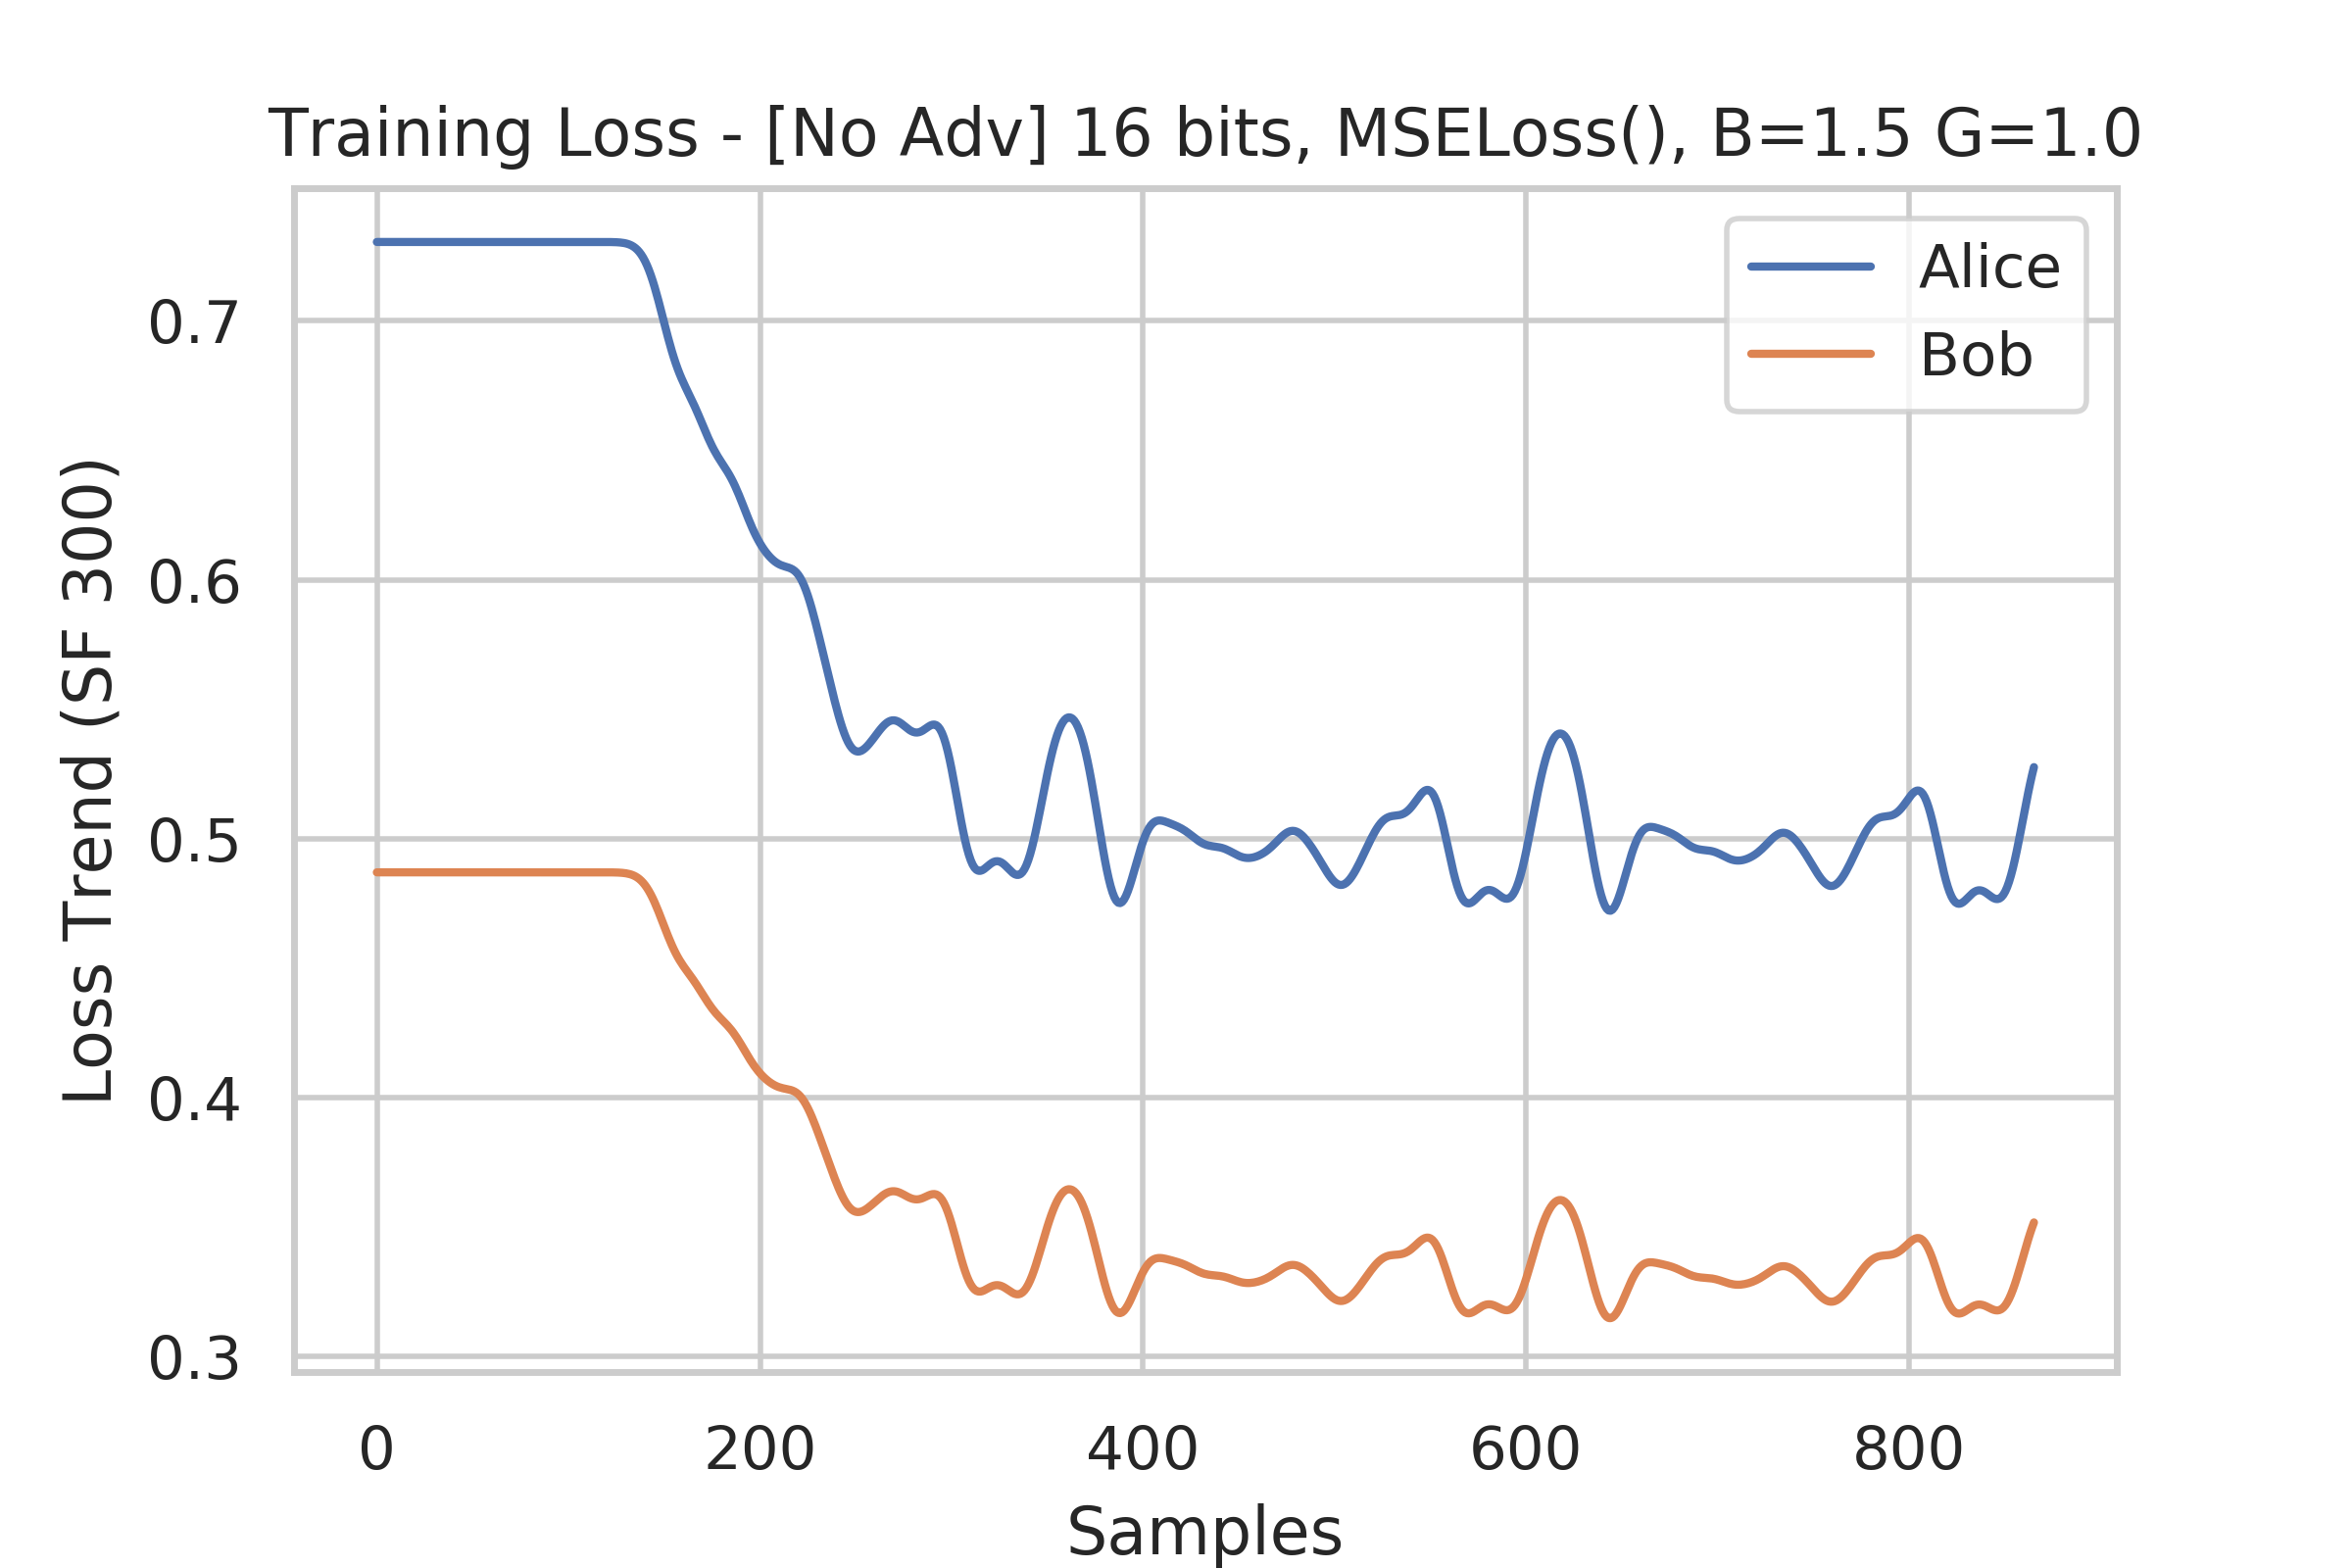
\includegraphics[width=0.48\textwidth]{../../models/cryptonet/graphs/loss_1E64x256v17.png}
    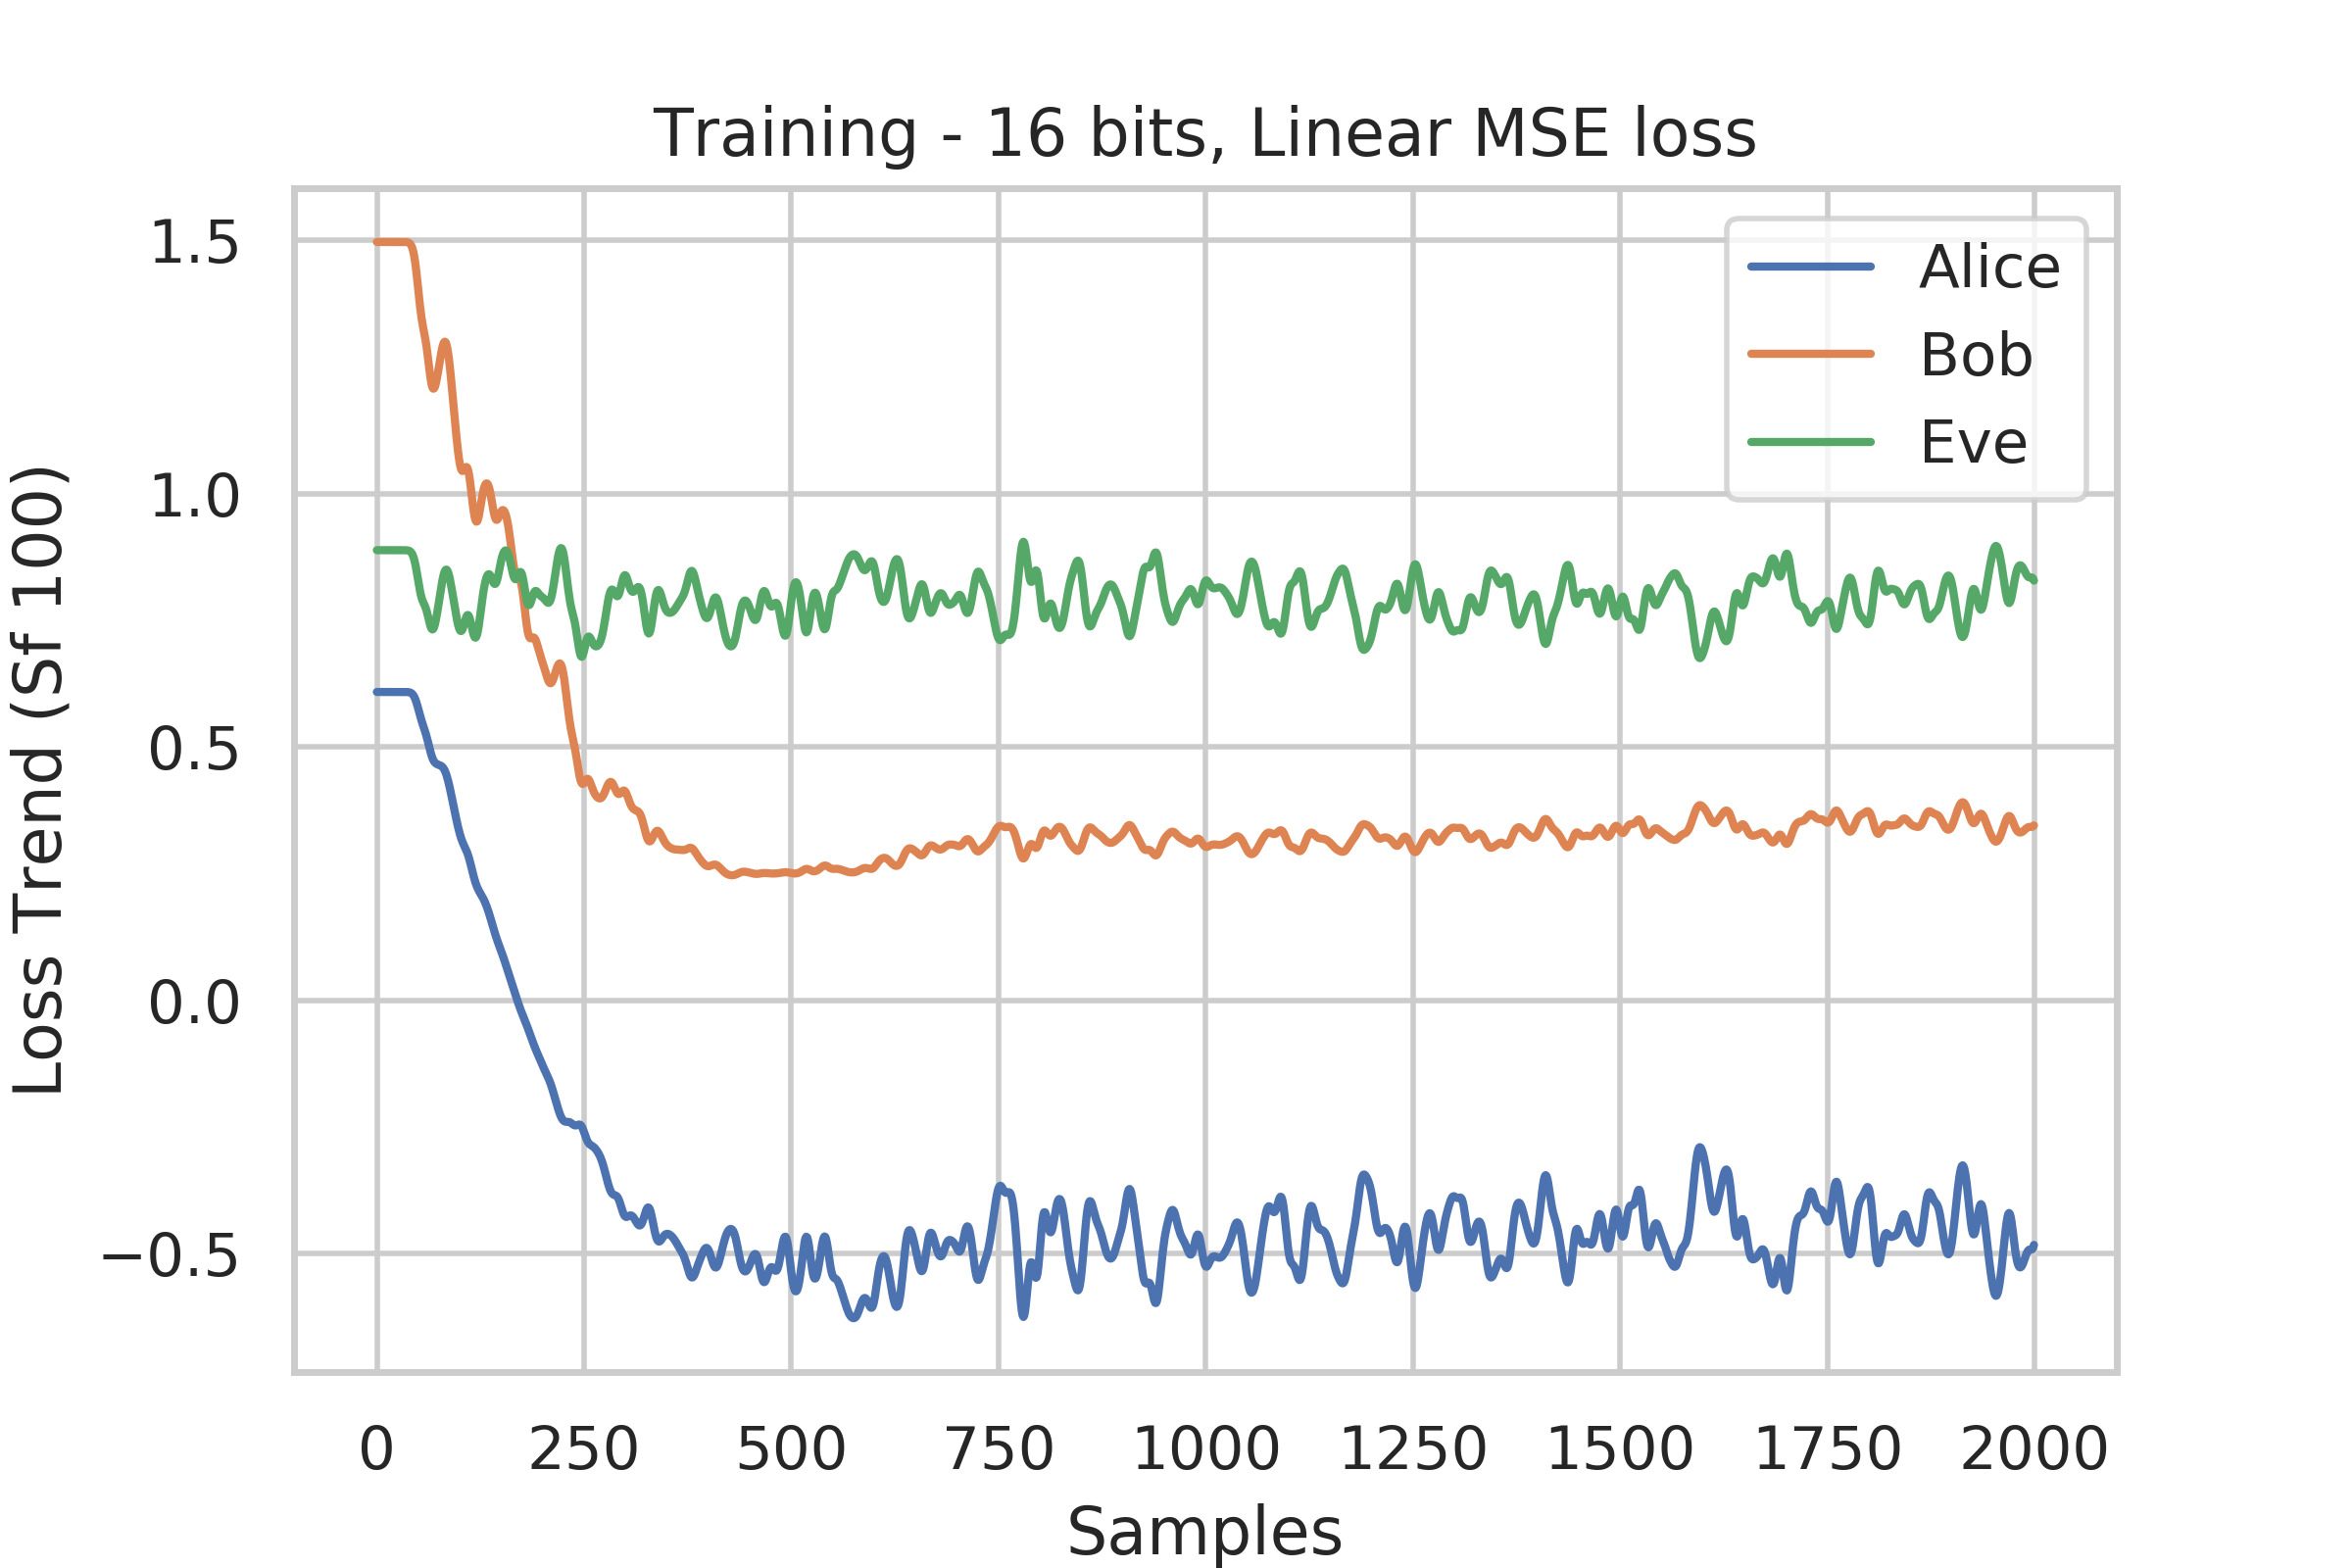
\includegraphics[width=0.48\textwidth]{../../models/anc/graphs/loss_1E2000v6.png}
    \caption{Loss Trend with ANC model by Abadi et al.}
    \label{fig:res_anc}
  \end{figure}

  \begin{center}
    \begin{tabular}{ c c c c }
      \hline
      \textbf{Key Size} & \textbf{Learning Rate} & \textbf{Epochs} & \textbf{Convergence} \\ \hline
      8 bits            & 0.0008                 & 8               & 4/10                 \\
      16 bits           & 0.0008                 & 10              & 4/10                 \\
      16 bits           & 0.0010                 & 16              & 6/10                 \\
      \hline
    \end{tabular}
  \end{center}
    
  The table above shows the number of times out of 10, that the networks converged with a 
  reasonable validation accuracy with different hyperparameters in the training.\\

  The following figures show the loss trends for the Cryptonet model with and without the adversary.
  Immediately we can notice that the rate of decrease of the loss is slower, which is a clear sign that
  the adversary Eve is having an effect on the training of Alice and Bob.

  \begin{figure}[H]
    \centering
    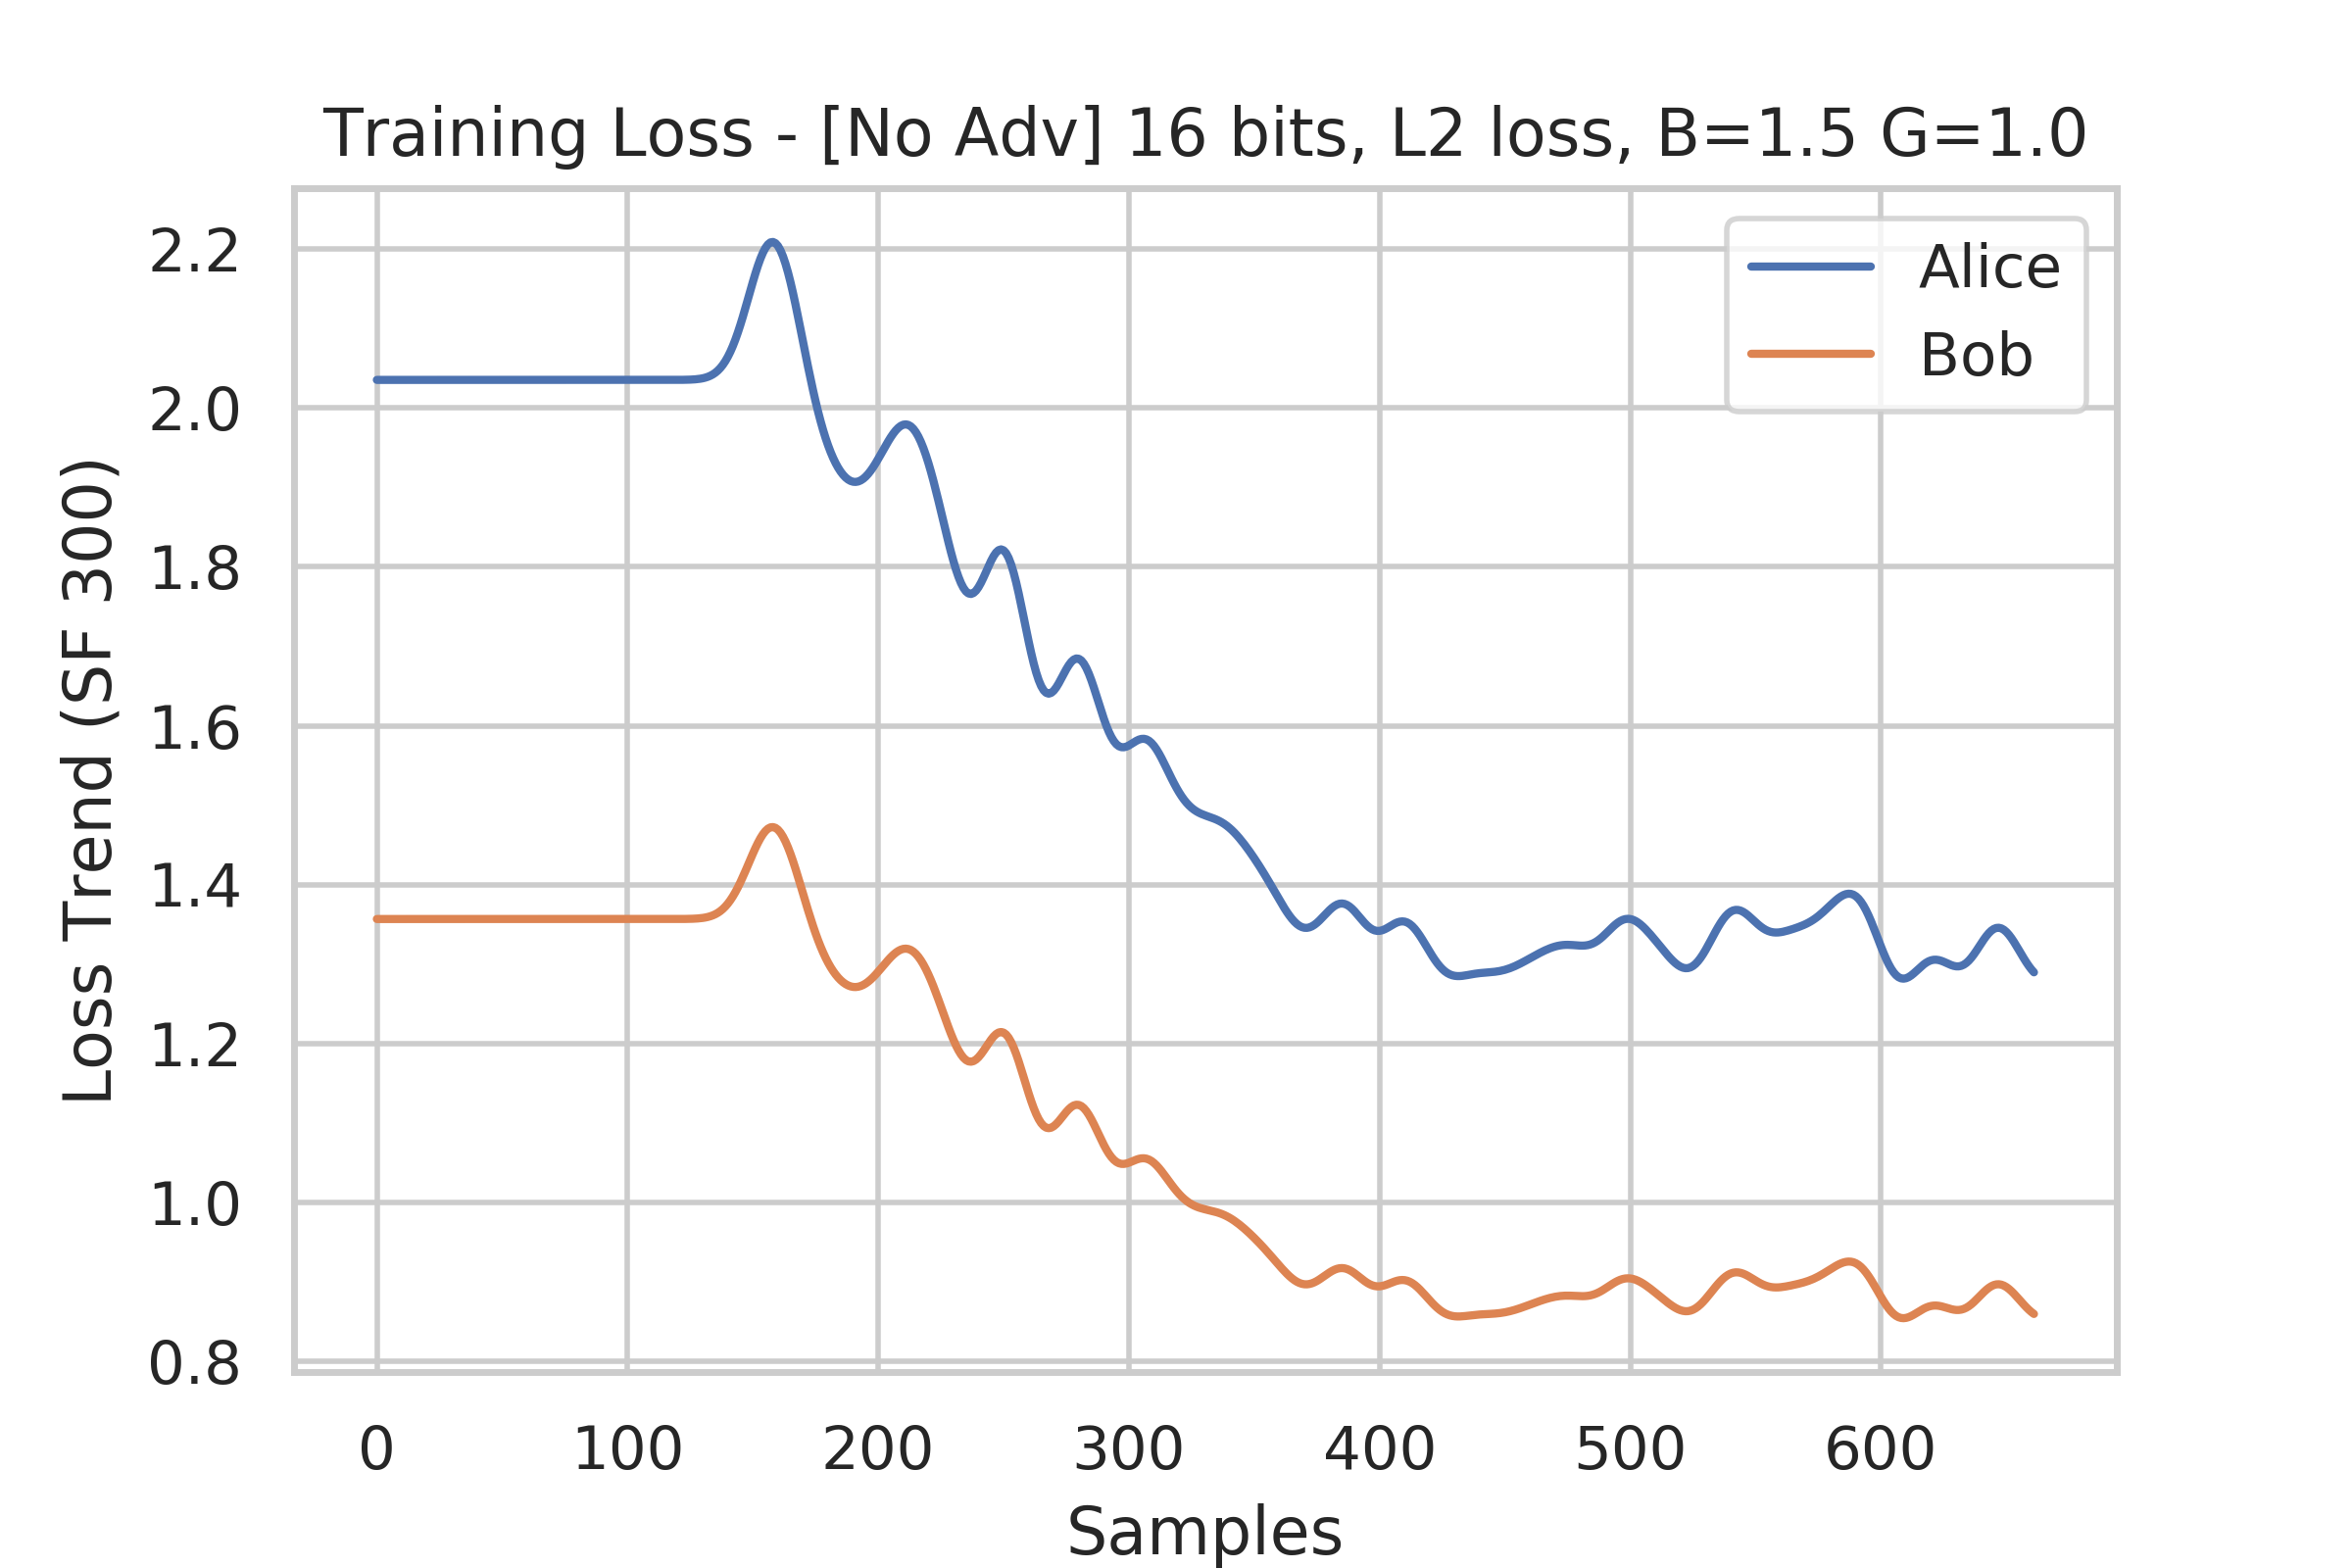
\includegraphics[width=0.48\textwidth]{../../models/cryptonet/graphs/loss_1E64x256v13.png}
    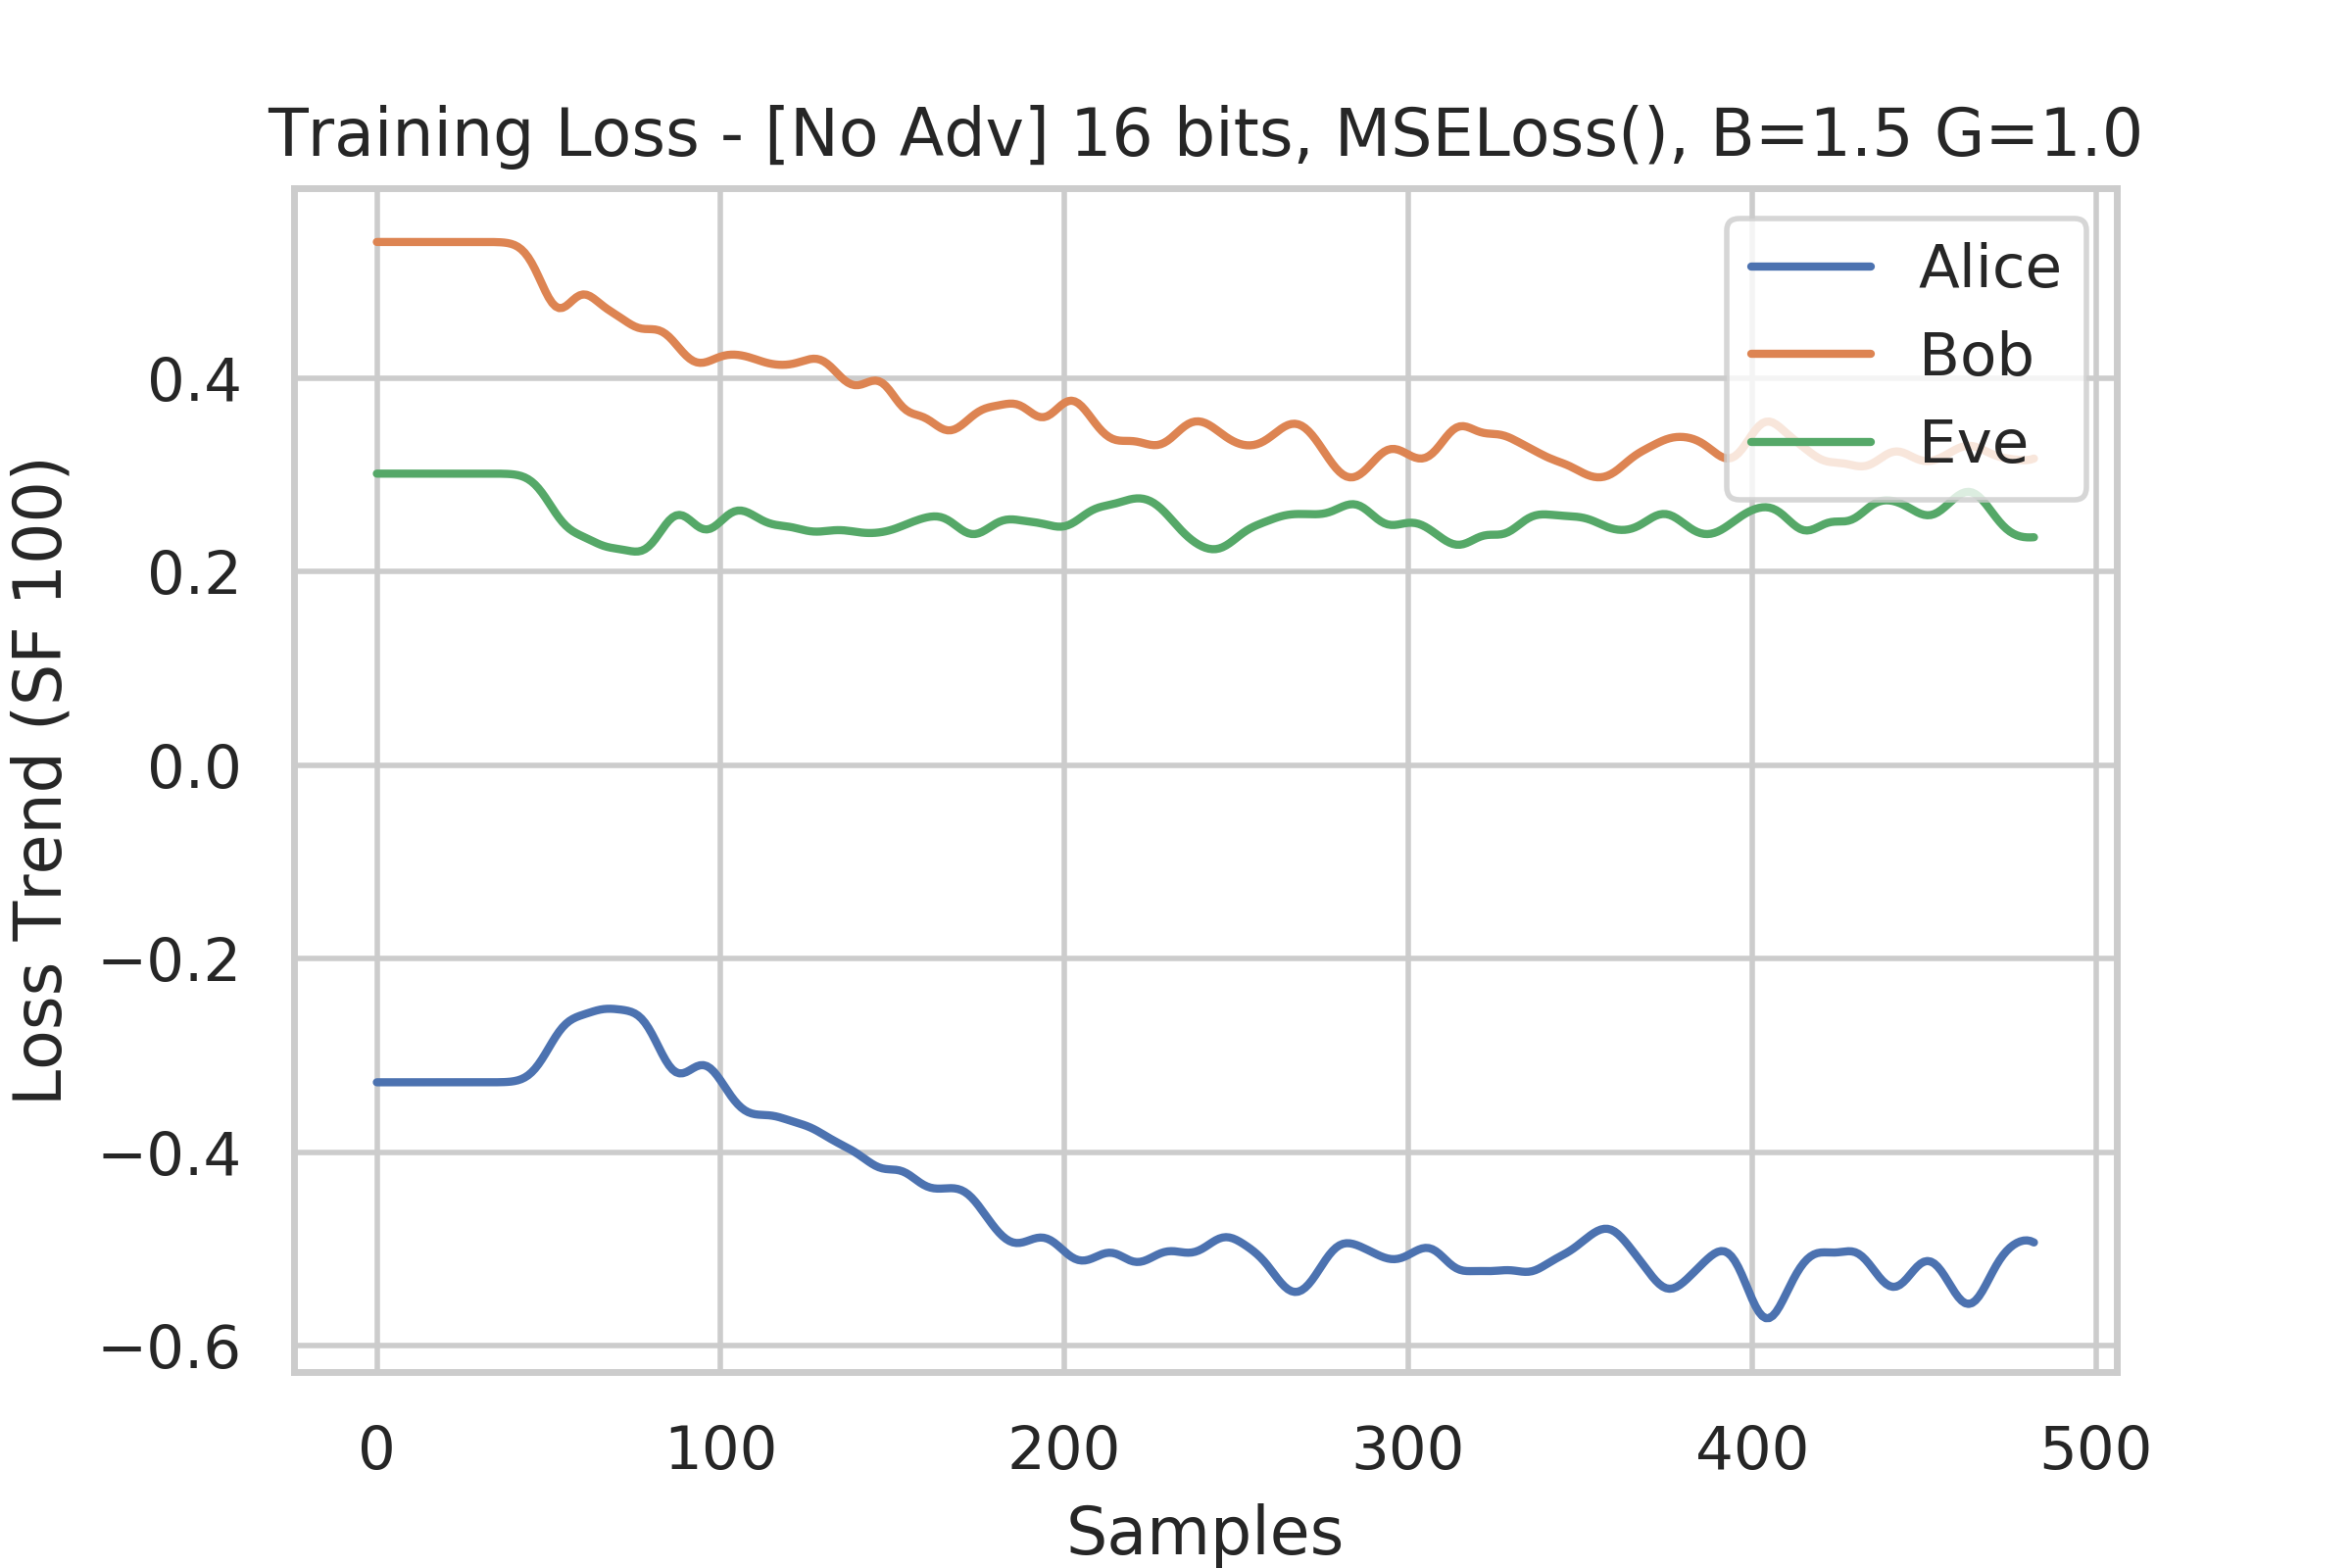
\includegraphics[width=0.48\textwidth]{../../models/cryptonet/graphs/loss_1E64x256v19.png}
    \caption{Loss Trend with Cryptonet model by Coutinho et al.}
    \label{fig:res_crnet}
  \end{figure}

  \begin{center}
    \begin{tabular}{ c c c c }
      \hline
      \textbf{Key Size} & \textbf{Learning Rate} & \textbf{Epochs} & \textbf{Convergence} \\ \hline
      4 bits            & 0.0008                 & 8               & 2/10                 \\
      8 bits            & 0.0008                 & 10              & 4/10                 \\
      8 bits            & 0.0008                 & 16              & 5/10                 \\
      \hline
    \end{tabular}
  \end{center}

    \pagebreak
    \subsection{Conclusion}
    In this project, we demonstrate that neural networks can learn to protect communications. The learning
    does not require prescribing a particular set of cryptographic algorithms, nor indicating ways
    of applying these algorithms: it is based only on a secrecy specification represented by the training
    objectives. In this setting, we model attackers by neural networks; alternative models may perhaps
    be enabled by reinforcement learning.

    There is more to cryptography than encryption. In this spirit, further work may consider other tasks,
    for example steganography, pseudorandom-number generation, or integrity checks. Finally, neural
    networks may be useful not only for cryptographic protections but also for attacks. While it seems
    improbable that neural networks would become great at cryptanalysis, they may be quite effective
    in making sense of metadata and in network traffic analysis.

    \subsection{Experimentation Areas}
    While this project had a reasonable level of success, there remains a lot of work to be done
    in this field. We will be examining the following areas of experimentation in the Major Project
    to take this further.
    \begin{enumerate}
      \item Using text embeddings and autoencoders in conjunction with these networks to produce 
      human readable ciphers from ordinary text.
      \item Investigating applications in end-to-end messaging and natural language to build 
      high-grade word substitution ciphers.
      \item Investigating the use of steganography in conjunction with an adversarial approach.
    \end{enumerate}

  % -------------------------------------------------------
  \newpage
  \section*{Bibliography}
  \addcontentsline{toc}{section}{Bibliography}
  \bibliographystyle{ieeetr}
  \bibliography{../../resources/citations}
  \listoffigures
\end{document}